% Options for packages loaded elsewhere
\PassOptionsToPackage{unicode}{hyperref}
\PassOptionsToPackage{hyphens}{url}
%
\documentclass[
]{book}
\usepackage{lmodern}
\usepackage{amsmath}
\usepackage{ifxetex,ifluatex}
\ifnum 0\ifxetex 1\fi\ifluatex 1\fi=0 % if pdftex
  \usepackage[T1]{fontenc}
  \usepackage[utf8]{inputenc}
  \usepackage{textcomp} % provide euro and other symbols
  \usepackage{amssymb}
\else % if luatex or xetex
  \usepackage{unicode-math}
  \defaultfontfeatures{Scale=MatchLowercase}
  \defaultfontfeatures[\rmfamily]{Ligatures=TeX,Scale=1}
\fi
% Use upquote if available, for straight quotes in verbatim environments
\IfFileExists{upquote.sty}{\usepackage{upquote}}{}
\IfFileExists{microtype.sty}{% use microtype if available
  \usepackage[]{microtype}
  \UseMicrotypeSet[protrusion]{basicmath} % disable protrusion for tt fonts
}{}
\makeatletter
\@ifundefined{KOMAClassName}{% if non-KOMA class
  \IfFileExists{parskip.sty}{%
    \usepackage{parskip}
  }{% else
    \setlength{\parindent}{0pt}
    \setlength{\parskip}{6pt plus 2pt minus 1pt}}
}{% if KOMA class
  \KOMAoptions{parskip=half}}
\makeatother
\usepackage{xcolor}
\IfFileExists{xurl.sty}{\usepackage{xurl}}{} % add URL line breaks if available
\IfFileExists{bookmark.sty}{\usepackage{bookmark}}{\usepackage{hyperref}}
\hypersetup{
  pdftitle={Best Coding Practices for R},
  pdfauthor={Vikram Singh Rawat},
  hidelinks,
  pdfcreator={LaTeX via pandoc}}
\urlstyle{same} % disable monospaced font for URLs
\usepackage{color}
\usepackage{fancyvrb}
\newcommand{\VerbBar}{|}
\newcommand{\VERB}{\Verb[commandchars=\\\{\}]}
\DefineVerbatimEnvironment{Highlighting}{Verbatim}{commandchars=\\\{\}}
% Add ',fontsize=\small' for more characters per line
\usepackage{framed}
\definecolor{shadecolor}{RGB}{248,248,248}
\newenvironment{Shaded}{\begin{snugshade}}{\end{snugshade}}
\newcommand{\AlertTok}[1]{\textcolor[rgb]{0.94,0.16,0.16}{#1}}
\newcommand{\AnnotationTok}[1]{\textcolor[rgb]{0.56,0.35,0.01}{\textbf{\textit{#1}}}}
\newcommand{\AttributeTok}[1]{\textcolor[rgb]{0.77,0.63,0.00}{#1}}
\newcommand{\BaseNTok}[1]{\textcolor[rgb]{0.00,0.00,0.81}{#1}}
\newcommand{\BuiltInTok}[1]{#1}
\newcommand{\CharTok}[1]{\textcolor[rgb]{0.31,0.60,0.02}{#1}}
\newcommand{\CommentTok}[1]{\textcolor[rgb]{0.56,0.35,0.01}{\textit{#1}}}
\newcommand{\CommentVarTok}[1]{\textcolor[rgb]{0.56,0.35,0.01}{\textbf{\textit{#1}}}}
\newcommand{\ConstantTok}[1]{\textcolor[rgb]{0.00,0.00,0.00}{#1}}
\newcommand{\ControlFlowTok}[1]{\textcolor[rgb]{0.13,0.29,0.53}{\textbf{#1}}}
\newcommand{\DataTypeTok}[1]{\textcolor[rgb]{0.13,0.29,0.53}{#1}}
\newcommand{\DecValTok}[1]{\textcolor[rgb]{0.00,0.00,0.81}{#1}}
\newcommand{\DocumentationTok}[1]{\textcolor[rgb]{0.56,0.35,0.01}{\textbf{\textit{#1}}}}
\newcommand{\ErrorTok}[1]{\textcolor[rgb]{0.64,0.00,0.00}{\textbf{#1}}}
\newcommand{\ExtensionTok}[1]{#1}
\newcommand{\FloatTok}[1]{\textcolor[rgb]{0.00,0.00,0.81}{#1}}
\newcommand{\FunctionTok}[1]{\textcolor[rgb]{0.00,0.00,0.00}{#1}}
\newcommand{\ImportTok}[1]{#1}
\newcommand{\InformationTok}[1]{\textcolor[rgb]{0.56,0.35,0.01}{\textbf{\textit{#1}}}}
\newcommand{\KeywordTok}[1]{\textcolor[rgb]{0.13,0.29,0.53}{\textbf{#1}}}
\newcommand{\NormalTok}[1]{#1}
\newcommand{\OperatorTok}[1]{\textcolor[rgb]{0.81,0.36,0.00}{\textbf{#1}}}
\newcommand{\OtherTok}[1]{\textcolor[rgb]{0.56,0.35,0.01}{#1}}
\newcommand{\PreprocessorTok}[1]{\textcolor[rgb]{0.56,0.35,0.01}{\textit{#1}}}
\newcommand{\RegionMarkerTok}[1]{#1}
\newcommand{\SpecialCharTok}[1]{\textcolor[rgb]{0.00,0.00,0.00}{#1}}
\newcommand{\SpecialStringTok}[1]{\textcolor[rgb]{0.31,0.60,0.02}{#1}}
\newcommand{\StringTok}[1]{\textcolor[rgb]{0.31,0.60,0.02}{#1}}
\newcommand{\VariableTok}[1]{\textcolor[rgb]{0.00,0.00,0.00}{#1}}
\newcommand{\VerbatimStringTok}[1]{\textcolor[rgb]{0.31,0.60,0.02}{#1}}
\newcommand{\WarningTok}[1]{\textcolor[rgb]{0.56,0.35,0.01}{\textbf{\textit{#1}}}}
\usepackage{longtable,booktabs}
\usepackage{calc} % for calculating minipage widths
% Correct order of tables after \paragraph or \subparagraph
\usepackage{etoolbox}
\makeatletter
\patchcmd\longtable{\par}{\if@noskipsec\mbox{}\fi\par}{}{}
\makeatother
% Allow footnotes in longtable head/foot
\IfFileExists{footnotehyper.sty}{\usepackage{footnotehyper}}{\usepackage{footnote}}
\makesavenoteenv{longtable}
\usepackage{graphicx}
\makeatletter
\def\maxwidth{\ifdim\Gin@nat@width>\linewidth\linewidth\else\Gin@nat@width\fi}
\def\maxheight{\ifdim\Gin@nat@height>\textheight\textheight\else\Gin@nat@height\fi}
\makeatother
% Scale images if necessary, so that they will not overflow the page
% margins by default, and it is still possible to overwrite the defaults
% using explicit options in \includegraphics[width, height, ...]{}
\setkeys{Gin}{width=\maxwidth,height=\maxheight,keepaspectratio}
% Set default figure placement to htbp
\makeatletter
\def\fps@figure{htbp}
\makeatother
\setlength{\emergencystretch}{3em} % prevent overfull lines
\providecommand{\tightlist}{%
  \setlength{\itemsep}{0pt}\setlength{\parskip}{0pt}}
\setcounter{secnumdepth}{5}
\usepackage{booktabs}
\ifluatex
  \usepackage{selnolig}  % disable illegal ligatures
\fi
\usepackage[]{natbib}
\bibliographystyle{apalike}

\title{Best Coding Practices for R}
\author{Vikram Singh Rawat}
\date{2021-03-26}

\begin{document}
\maketitle

{
\setcounter{tocdepth}{1}
\tableofcontents
}
\hypertarget{part-introduction}{%
\part{Introduction}\label{part-introduction}}

\begin{Shaded}
\begin{Highlighting}[]
\NormalTok{knitr}\SpecialCharTok{::}\NormalTok{opts\_chunk}\SpecialCharTok{$}\FunctionTok{set}\NormalTok{(}\AttributeTok{include =} \ConstantTok{TRUE}\NormalTok{)}

\FunctionTok{library}\NormalTok{(magrittr)}
\FunctionTok{library}\NormalTok{(quanteda)}
\end{Highlighting}
\end{Shaded}

\begin{verbatim}
## Warning: package 'quanteda' was built under R version 4.0.3
\end{verbatim}

\begin{verbatim}
## Package version: 2.1.2
\end{verbatim}

\begin{verbatim}
## Parallel computing: 2 of 8 threads used.
\end{verbatim}

\begin{verbatim}
## See https://quanteda.io for tutorials and examples.
\end{verbatim}

\begin{verbatim}
## 
## Attaching package: 'quanteda'
\end{verbatim}

\begin{verbatim}
## The following object is masked from 'package:utils':
## 
##     View
\end{verbatim}

\begin{Shaded}
\begin{Highlighting}[]
\FunctionTok{library}\NormalTok{(dplyr)}
\end{Highlighting}
\end{Shaded}

\begin{verbatim}
## 
## Attaching package: 'dplyr'
\end{verbatim}

\begin{verbatim}
## The following objects are masked from 'package:stats':
## 
##     filter, lag
\end{verbatim}

\begin{verbatim}
## The following objects are masked from 'package:base':
## 
##     intersect, setdiff, setequal, union
\end{verbatim}

\hypertarget{coverpage}{%
\chapter*{CoverPage}\label{coverpage}}
\addcontentsline{toc}{chapter}{CoverPage}

\begin{quote}
Know the rules well, so you can break them effectively.
--- The Dalai Lama
\end{quote}

\begin{center}\rule{0.5\linewidth}{0.5pt}\end{center}

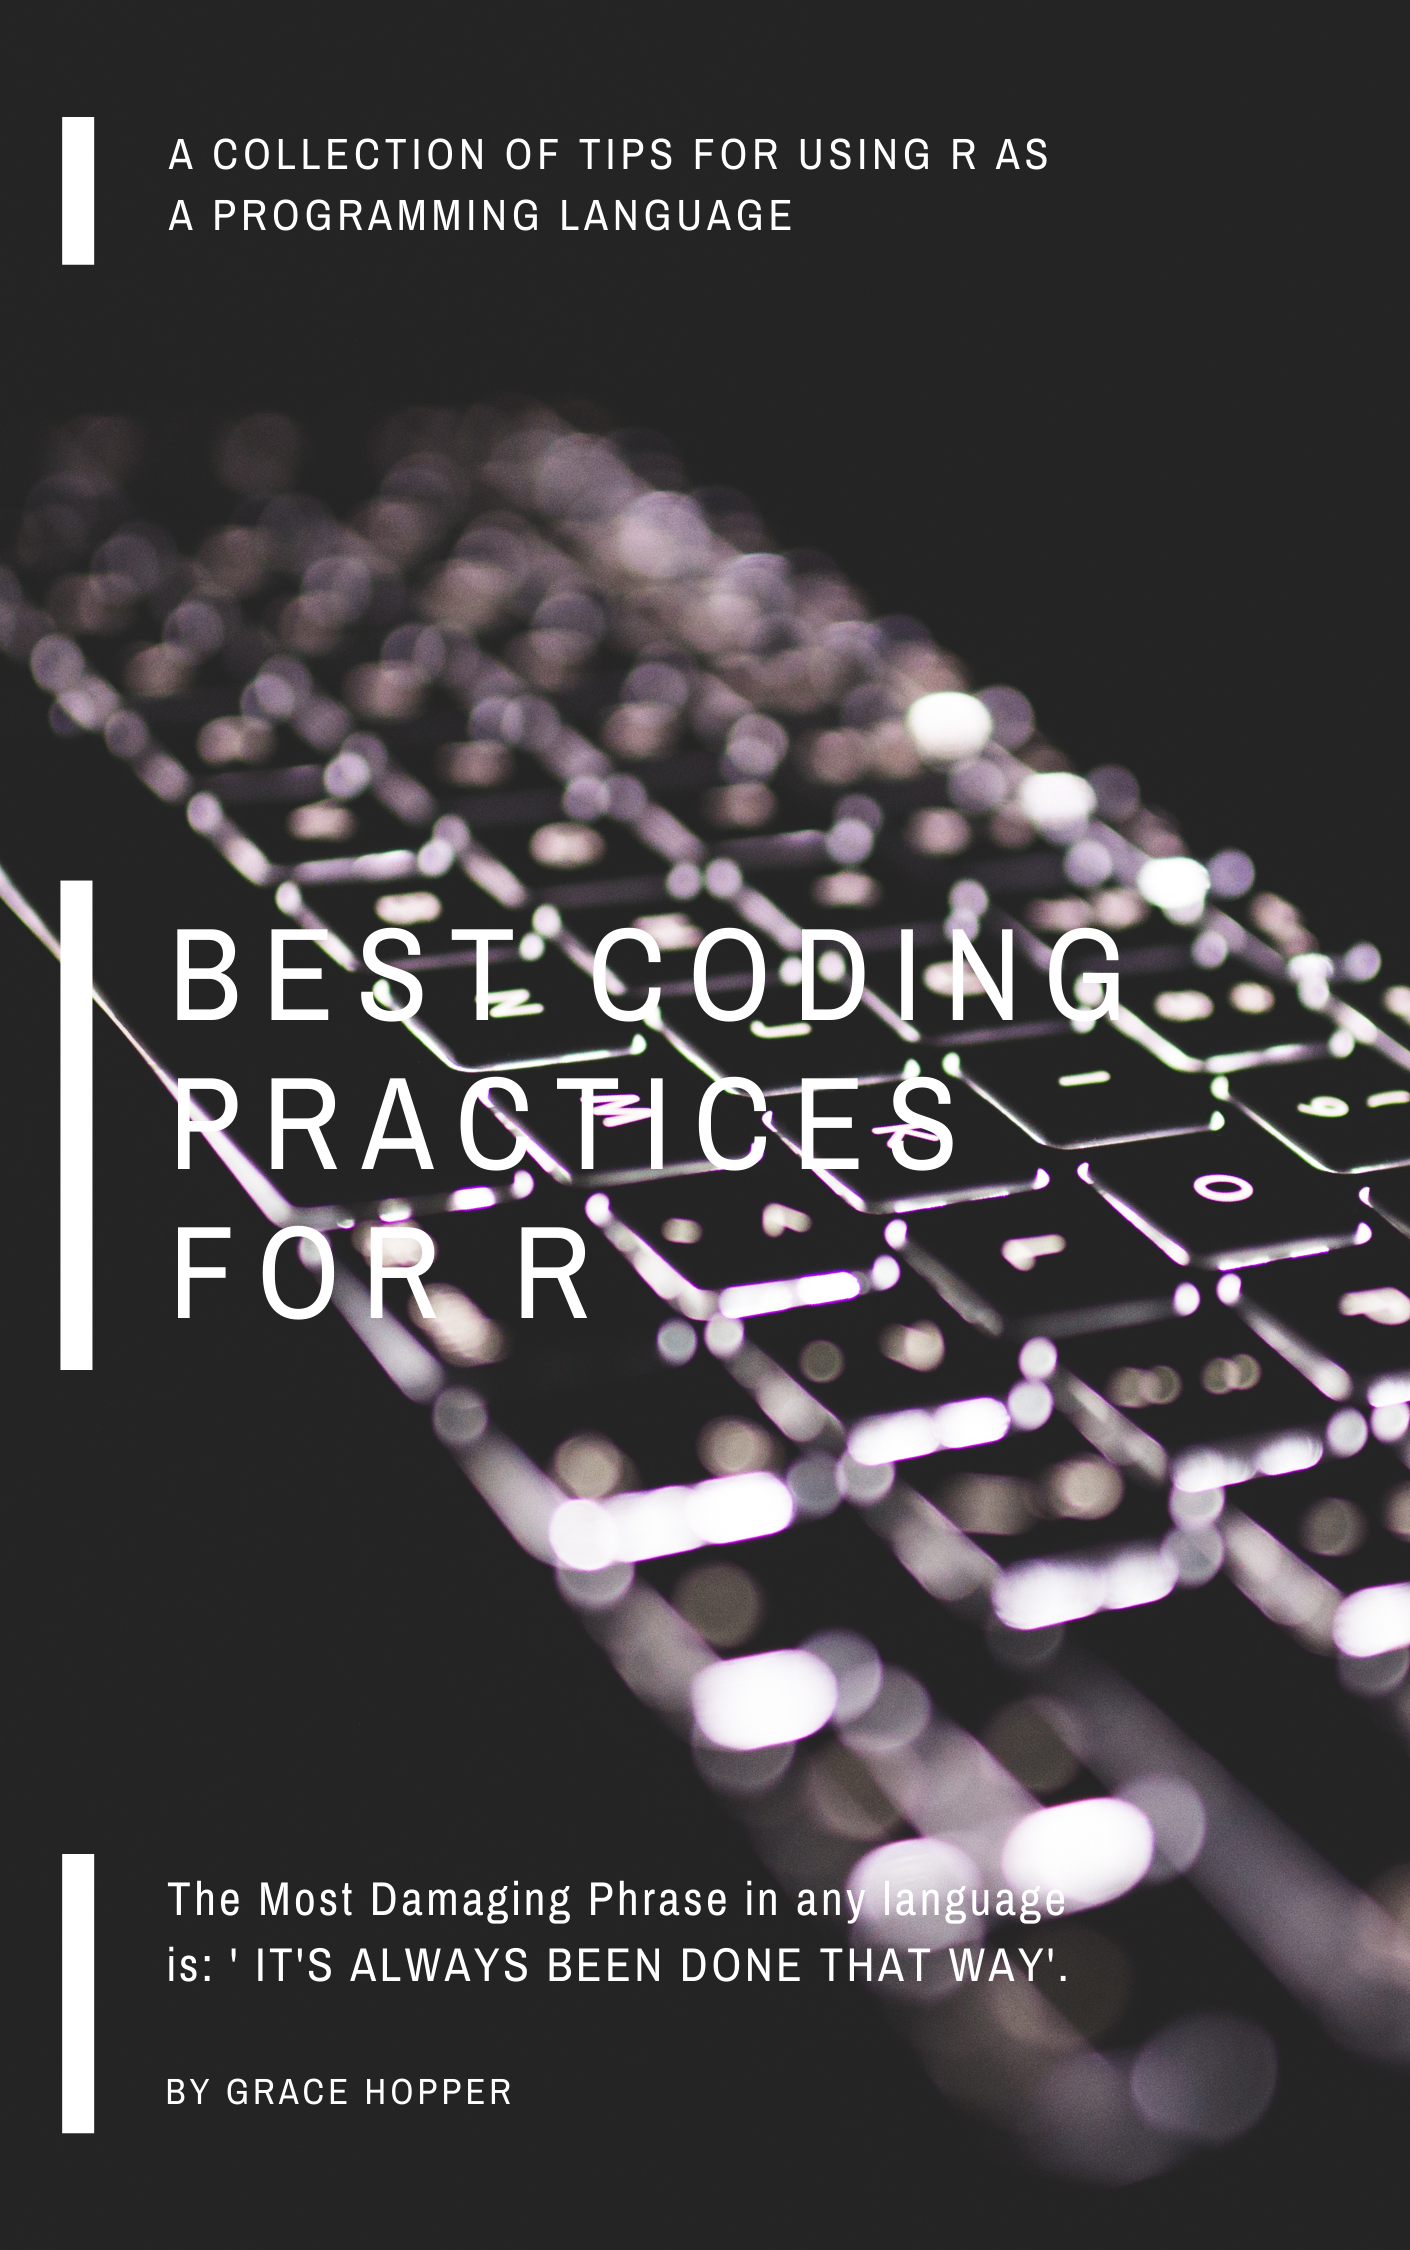
\includegraphics{figures/cover.png}

\hypertarget{intro}{%
\chapter{Introduction}\label{intro}}

\begin{quote}
\begin{itemize}
\tightlist
\item
  The most damaging phrase in the language is: 'It's always been done that way.*.
\end{itemize}

--- Grace Hopper
\end{quote}

\begin{center}\rule{0.5\linewidth}{0.5pt}\end{center}

Did you try to read the title from the cover of the book? I could have done a thousand things to make it easier for you to read it. But this cover reminds me of how often we overlook simple things which are very crucial from the reader's point of view.

R is an excellent programming language it's turing complete and doesn't lack anything for a production level code. It can be used in the entire data domain from API's to dashboards to apps and much more. Trust the language and trust in yourself. It's a journey everyone has gone through and everyone must go through.

R programmers have a bad reputation for not writing production level code. It stems from the fact that we mostly aren't trained programmers. We tend to overlook things that are crucial from a programming standpoint. As R programmers we are often less inclined to write the code for production. Mostly we try to write scripts and when we are asked to deploy the same we just wrap it in a function and provide it to the IT team. I have been at the receiving end of these issues where I had to maintain a poorly written code; \textbf{columns were referred by numbers, functions were dependent upon global environment variables, 50+ lines functions without arguement, poor naming conventions etc\ldots{}}.

I too am a self taught programmer and have gone through these hiccups of code deployment, code reviews and speed issues. World going forward will all be code and data. The sooner you learn these skills the better it is for you to have trust in your own programming skills. R is a huge language and I would like to share the little knowledge I have in the subject. I don't claim to be an expert but this book will guide you in the right path wherever possible.

\emph{\textbf{Most of the books about R programming language will tell you what are the possible ways to do one thing in R. This book will only tell you one way to do that thing correctly}.}

I will try to write it as a dictionary as succinctly as possible. So that you can use it for references. Let the journey begin\ldots{}

\hypertarget{part-structure}{%
\part{Structure}\label{part-structure}}

\hypertarget{folder}{%
\chapter{Folder Structure}\label{folder}}

\hypertarget{organizing-files}{%
\section{Organizing files}\label{organizing-files}}

\begin{quote}
The best way to organize your code is to write a \textbf{package}.
\end{quote}

Organizing your code is the first and foremost thing you should learn. Because as the project grows and multiple files are put into a folder it gets harder to navigate the code. A proper folder structure definitely helps in these times. I Just couldn't emphasis it enough that best way to organize your code is to write a package. But even when you are not planning to write a package. There are best practices to make it readable and make a smooth navigation.

\hypertarget{create-projects}{%
\section{Create Projects}\label{create-projects}}

It's such a minor thing to say but I still till date see code like this:

\begin{verbatim}
setwd("c://myproject_name/")
\end{verbatim}

It was a good practice like 5 - 6 years ago. Now Rstudio has a feature to create project.

\begin{figure}
\centering
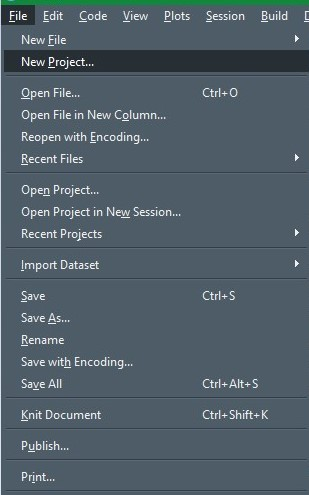
\includegraphics{./figures/scrn_new_project.jpg}
\caption{new project}
\end{figure}

Once you create a project it is easier to manage your files and folders and it's easier to give it somebody as well. It has virtually the same effect but then you can use Rstudio a little better. It's something I recommend to every user regardless of the skill level.

\hypertarget{naming-files}{%
\section{Naming files}\label{naming-files}}

I data science most common problem is that we don't change the file names of excel or csv files provided by business people. And most of the time those file names are totally abbreviated with spaces in between and multiple cases like \texttt{Total\ Sales\ Mike\ 202002-AZ1P2R.csv}. This name is useful for the MIS or Business Analyst as they have a different way of organizing files then yours. They might do it because they have to keep a record of different people and have to provide it anytime asked. But as a Data Scientist your work is entirely different. You are not delivering files you are writing code. Let me reiterate this fact \textbf{YOU ARE WRITING CODE}. In most of the scenarios \textbf{Data Science is more like programming less like science}. Even though it has proportion of both of them. Using fundamentals of programming practices will help you out in long term. So change such file names to \texttt{sales\_data\_mike\_feb2020.csv} or something similar. There are no right or wrong names just what makes more sense to a new user.

There is a trick about naming conventions:

\begin{enumerate}
\def\labelenumi{\arabic{enumi}.}
\tightlist
\item
  use all lower case or upper case ( helps you in never forgetting the cases )
\item
  use underscore in between ( Because file names are mostly long Camel Or Pascal cases may confuse users)
\item
  make the name as general as possible ( make sure a newcomer should be able to understand it without any problem)
\item
  In choosing a name there are no wrong answers only confusing ones
\end{enumerate}

\hypertarget{folders-based-on-file-type}{%
\section{Folders Based on File-Type}\label{folders-based-on-file-type}}

A Very common practice is to keep different file types in different folder. One of the main mistake I see people writing code like this.

\begin{verbatim}
DBI::dbGetQuery(conn,
"
select 
    count(*) as numbers,
    max(colname) as maxSome,
    min(colname) as minSome,
  from
    tablename
  group by
    col1,
    col2,
    col3
  order by 
    numbers
")
\end{verbatim}

or codes like this.

\begin{verbatim}
shiny::HTML(
"
   <p>At Mozilla, we’re a global community of</p>

    <ul> <!-- changed to list in the tutorial -->
      <li>technologists</li>
      <li>thinkers</li>
      <li>builders</li>
    </ul>

    <p>working together to keep the Internet alive and accessible, so people worldwide can be informed contributors and creators of the Web. We believe this act of human collaboration across an open platform is essential to individual growth and our collective future.</p>

    <p>Read the <a href=\"https://www.mozilla.org/en-US/about/manifesto/\">Mozilla Manifesto</a> to learn even more about the values and principles that guide the pursuit of our mission.</p>
"
)
\end{verbatim}

This is a bad coding style. Every time I see this type of code I realize that the person doesn't believe that either the code will change or It will be extended. \textbf{\emph{There is nothing permanent in the programming}} neither code, nor frameworks and not even languages. If you keep this type of code in separate SQL files or html files you can easily edit them later, code will be more easier to read and there will be a separation of concern. Tomorrow if you need help in SQL or HTML, a UI designer or a Database designer can look into your code without getting bogged down in R code. It makes bringing more people to the team easier.

\hypertarget{creating-sub-folders}{%
\section{Creating Sub-folders}\label{creating-sub-folders}}

On bigger projects simple folder structure tend to become more confusing. This is the main concern I have with the data folder every data scientist create and put all the files he has in that single folder. In these scenarios it's better to have a sub-folder for different file types or may be different roles.

Like you can create sub-folders based on file-types like CSV's, json, rds etc.. or you can even create sub-folders based on roles or needs\ldots{} Like all the data related to one tab or one functionality goes in one folder and so on\ldots{} There has to be a logical consistency in the folder structure. It's primarily for you to not get lost in your own folders that you created and secondary for people working with you to understand your code and help in places you need help.

\hypertarget{conclusion}{%
\section{Conclusion}\label{conclusion}}

You have to create folders and everything has to be arranged in. Keep everything as organized as you keep your house. There are a certain principles that will help you in it.

\begin{enumerate}
\def\labelenumi{\arabic{enumi}.}
\tightlist
\item
  Create projects
\item
  Name the files properly
\item
  Create a file for different language
\item
  create sub-folders wherever you fill necessary.
\end{enumerate}

\hypertarget{code}{%
\chapter{Code Structure}\label{code}}

Once you have arranged the files and folders in a logical way then comes the fact that the code itself should be arranged in such a way that it feels easy to go through. Always remember \textbf{Code is read more often then it's written}. Your world should revolve around this line. If you delegate your work while leaving your firm to someone else than the person who is handling your code should be able to understand everything you were trying to do. You will be in that position someday and you would wish your colleagues must have done the same. Even if you aren't sharing your code to somebody one day when you will return back to the project after say 7 to 8 months you will be surprised to see the mess you created back then. With this in mind hope this will help you in your journey.

\hypertarget{create-sections}{%
\section{Create Sections}\label{create-sections}}

Rstudio gives you an ability to create section by pressing ( ctrl + shift + R ), or you can create one

by adding 4 dashes (-) after a comment or 4 hash symbol (\#) after a comment.

\begin{verbatim}
# some comment ----
# some comment ####
\end{verbatim}

Both are valid syntax. you can name your section in the comment. Same rule applies for the Rmarkdown documents as well you should always name your code chunk.

\begin{verbatim}
# ```{r chunkname, cache=TRUE}
\end{verbatim}

It also helps you jump between sections (Shift+Alt+J). You can easily switch between sections and fold them at will. It helps you not only in navigation but keeping a layout of the entire code as well.

A 800+ line files will look something like this.

\begin{figure}
\centering
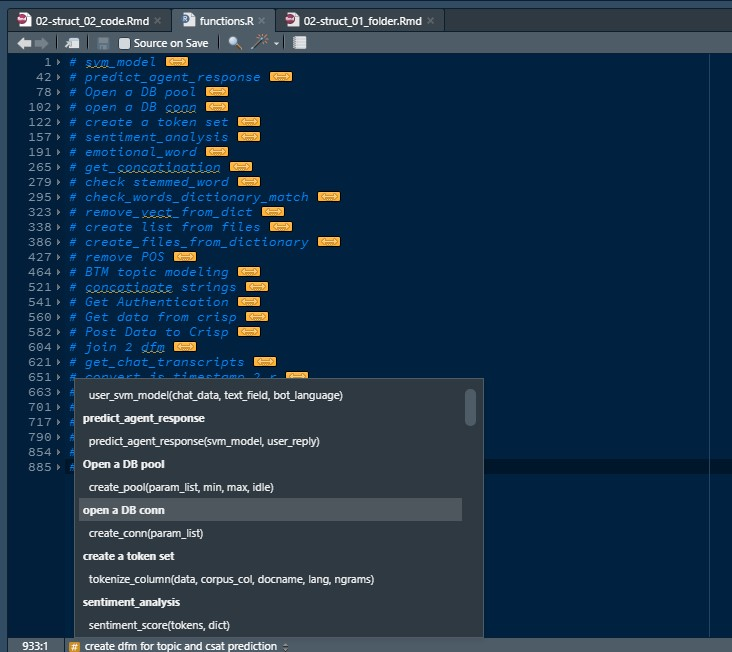
\includegraphics{./figures/scrn_sections.jpg}
\caption{code chunk}
\end{figure}

It makes your code beautiful to look and makes it maintainable in long run.

\hypertarget{order-of-code}{%
\section{Order of Code}\label{order-of-code}}

When you write code there are standard practices that are used across the domain and you should definitely use them. These are simple rules that most beginners aren't concerned about but the more experience you gain the more you start to realize the latent power of code organization. Here are a simple tip you should use.

\begin{enumerate}
\def\labelenumi{\arabic{enumi}.}
\tightlist
\item
  Call your libraries on top of code
\item
  Set all default variables or global options and all the path variables at the top of the code.
\item
  Source all the code at the beginning
\item
  Call all the data-files at the top
\end{enumerate}

In this exact order. This coherence keeps all your code easy to find. Most annoying thing in debugging someone else code is finding path variables laid out inside functions. Please don't ever do that. That is not a good practices. Take a look at one of my file

\begin{figure}
\centering
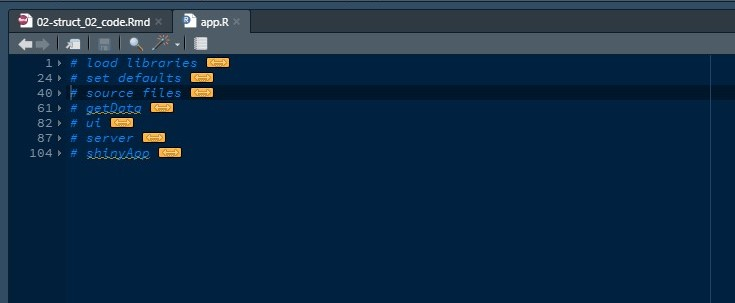
\includegraphics{./figures/scrn_section_order.jpg}
\caption{code order}
\end{figure}

If you think you will forget it. There is a golden rule you must remember. \textbf{\emph{Put all the external dependencies on top of your code}}. Everything that I mentioned above is external to the code in the file. In exact order.

\begin{enumerate}
\def\labelenumi{\arabic{enumi}.}
\tightlist
\item
  Libraries are external to the file.
\item
  path variables
\item
  other files apart from one you are working is external as well.
\item
  databases and CSV
\end{enumerate}

Just by doing this you will be able to navigate better in your code. There aren't any hard and fast rules for this only logical and sensible ones. Feel free to come up with your own layout that helps you in your analysis journey.

\hypertarget{indentation}{%
\section{Indentation}\label{indentation}}

It goes without saying that indentation makes your code readable. Python is not the only language who has the luxury of indentation. No matter what language you work in your code should be properly indented so that we can understand the nature of code written. There are a few things you can understand about indentation.

Maintain same number of spaces throughout your code. Your editor will help you out with it for sure but even if you are working on multiple editors. If you choose 2 spaces or 4 spaces as an equivalent of tabs you should stick to it. This is a golden rule you should never break.

Then maintain the same style in your code. Look at the code below.

\begin{Shaded}
\begin{Highlighting}[]
\NormalTok{foo }\OtherTok{\textless{}{-}} \ControlFlowTok{function}\NormalTok{(}
\NormalTok{  first\_arg, second\_arg, third\_arg}
\NormalTok{)\{}
\NormalTok{  create\_file }\OtherTok{\textless{}{-}}\NormalTok{ readxl}\SpecialCharTok{::}\FunctionTok{read\_excel}\NormalTok{(}\AttributeTok{path =}\NormalTok{ first\_arg, }\AttributeTok{sheet =}\NormalTok{ second\_arg, }
                                    \AttributeTok{range =}\NormalTok{ third\_arg)}
\NormalTok{\}}

\NormalTok{bar }\OtherTok{\textless{}{-}} \ControlFlowTok{function}\NormalTok{(}
\NormalTok{  first\_arg,}
\NormalTok{  second\_arg,}
\NormalTok{  third\_arg}
\NormalTok{)\{}
\NormalTok{  create\_file }\OtherTok{\textless{}{-}}\NormalTok{ readxl}\SpecialCharTok{::}\FunctionTok{read\_excel}\NormalTok{(}
    \AttributeTok{path =}\NormalTok{ first\_arg, }
    \AttributeTok{sheet =}\NormalTok{ second\_arg, }
    \AttributeTok{range =}\NormalTok{ third\_arg}
\NormalTok{    )}
\NormalTok{\}}
\end{Highlighting}
\end{Shaded}

function foo is written horizontal and bar is written vertical. I would prefer styling of function bar but you may choose one and stick to it for entire project. Mixing styles is not considered good and might create problem in code review.

There is a package by name \texttt{grkstyle} which implements vertical arrangement of code as mentioned above. You can look into it as well.

\hypertarget{conclusion-1}{%
\section{Conclusion'}\label{conclusion-1}}

In this chapter we discussed how to structure your code to make it more meaningful to read and easier to debug. The key takeaways from this chapter is:

\begin{enumerate}
\def\labelenumi{\arabic{enumi}.}
\tightlist
\item
  Create sections to write beautiful and navigable code
\item
  Put those sections in a logical order
\item
  Don't
\end{enumerate}

\hypertarget{func}{%
\chapter{Functions}\label{func}}

I can not over emphasize the importance of functions. As a data scientist most of the time you will be writing functions. Only in couple of cases where you have to write complicated classes there too methods are nothing more than functions. Having solid grasp of best practices in functions is a must for everybody working in any language what-so-ever. Hopefully this chapter will help you in best coding practices for functions.

\hypertarget{metadata-or-information-header}{%
\section{Metadata or Information header}\label{metadata-or-information-header}}

As I mentioned in the previous chapter it is a good practice to create sections for everything you do in R. functions are no exception to the rule. But along with that there are a couple of information you should write along with the function.

I worked in a few MNC where we had to write metadata of every function before writing it down. It makes it easier for code-reviewer to understand you code and for the entire team to collaborate in the project. It's good for personal projects too\ldots{} Let me give you an example of what I mean by this.

\begin{figure}
\centering
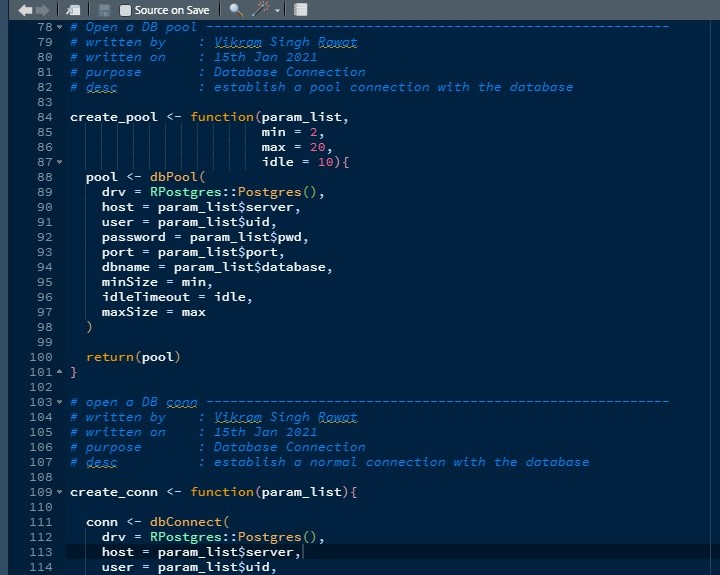
\includegraphics{./figures/scrn_functions_metadata.jpg}
\caption{functions metadata}
\end{figure}

You can see that if you are working on large teams or may be in big corporate settings where anybody can be reassigned to a different project. This data helps by identifying who wrote what and why.

Examples of some important tags can be :

\begin{enumerate}
\def\labelenumi{\arabic{enumi}.}
\tightlist
\item
  written by
\item
  written on
\item
  modified by
\item
  modified on
\item
  purpose
\item
  descriptions
\end{enumerate}

You can create your own tags based on usecases and information needed for further scenarios.

\hypertarget{pass-everything-through-parameters}{%
\section{Pass everything through parameters}\label{pass-everything-through-parameters}}

I have seen people writing functions with calling things from global environments. Take a look at the code below.

\begin{Shaded}
\begin{Highlighting}[]
\NormalTok{foo }\OtherTok{\textless{}{-}} \ControlFlowTok{function}\NormalTok{(x)\{}
   \FunctionTok{return}\NormalTok{( x }\SpecialCharTok{+}\NormalTok{ y)}
\NormalTok{\}}

\NormalTok{y }\OtherTok{\textless{}{-}} \DecValTok{10}

\FunctionTok{foo}\NormalTok{(}\DecValTok{5}\NormalTok{)}
\end{Highlighting}
\end{Shaded}

\begin{verbatim}
## [1] 15
\end{verbatim}

Here the value of \emph{foo} is based on y which is not a part of the function instead it's in global environment and function always have to search global environment for the object. consider these scenarios:

\begin{Shaded}
\begin{Highlighting}[]
\NormalTok{bar }\OtherTok{\textless{}{-}} \ControlFlowTok{function}\NormalTok{(x, y)\{}
\NormalTok{  y }\OtherTok{\textless{}{-}}\NormalTok{ y}
  \FunctionTok{return}\NormalTok{(}
    \FunctionTok{foo}\NormalTok{(x)}
\NormalTok{  )}
\NormalTok{\}}

\FunctionTok{bar}\NormalTok{(}\DecValTok{5}\NormalTok{, }\DecValTok{20}\NormalTok{)}
\end{Highlighting}
\end{Shaded}

\begin{verbatim}
## [1] 15
\end{verbatim}

you would assume that the answer is 25 but it's 15 because foo was created in the global environment and it will always look up value in global environment before anything else. This is called \textbf{Lexical Scoping} it's okay if you don't know it. It is very confusing and could mess up your code at any point in time. I am an experienced R programmer I too have trouble getting my head around it.

We can avoid all these situations by following the best coding practices that have been used in software industries for years. \textbf{Function should be a self contained code} which shouldn't be impacted by the outer world. Only is certain scenarios you allow to deviate from these rules but it's a good coding practice none the less. now in the above example instead of relying on the global variable if I just had created a parameter for Y, my code would be simpler to write and easier to understand and I would not have to think about lexical scoping on every step.

\begin{Shaded}
\begin{Highlighting}[]
\NormalTok{foo }\OtherTok{\textless{}{-}} \ControlFlowTok{function}\NormalTok{( x, y )\{}
   \FunctionTok{return}\NormalTok{( x }\SpecialCharTok{+}\NormalTok{ y )}
\NormalTok{\}}


\NormalTok{bar }\OtherTok{\textless{}{-}} \ControlFlowTok{function}\NormalTok{( x, y )\{}
  \FunctionTok{return}\NormalTok{(}
    \FunctionTok{foo}\NormalTok{( x, y )    }
\NormalTok{  )}
\NormalTok{\}}

\FunctionTok{bar}\NormalTok{(}\DecValTok{5}\NormalTok{, }\DecValTok{20}\NormalTok{)}
\end{Highlighting}
\end{Shaded}

\begin{verbatim}
## [1] 25
\end{verbatim}

Now this code returns 25 as we all expected and trust me the Y is still available in global environment but that doesn't impact the foo or bar at all. Now you can nest this function under multiple other functions and it will behave exactly like it should.

There is a golden rule you should take away from this section. \textbf{Avoid Global Variables at all costs}. As much as possible pass everything through the parameters. That what they are for right !!!

\hypertarget{use-return-statement}{%
\section{Use Return Statement}\label{use-return-statement}}

It is a very simple thing yet most of the R users never worry about it because R takes care of finer details for you. But return statements actually make your code easier to read.

Suppose you have to review code return statement makes it easier to glance at the code and understand what is it doing. Almost all the programming languages are habitual with it. There are no good advantage I can tell you for a return statement other than readability. But just by following these practices R community as a whole could get more respect in programming community. So please use Return statements wherever possible. In Big MNC your code will never pass reviewer unless it has return statements.

It also is good for functions that don't return anything you can just return true or false depending on the fact that the function ran without producing any error. Functions where you modify a data.table or where you change something in the database etc\ldots{} It's a standard practice in old programming languages like C++ and it's a good practice indeed. We as a community should embrace these practices which will help us down the road.

\hypertarget{keep-a-consistency-in-return-type}{%
\section{Keep a consistency in Return Type}\label{keep-a-consistency-in-return-type}}

\textbf{Return type of a function should be consistent regardless of what happens in a code.} You may assume this is so simple that it goes without saying who would in their sane mind return character vector instead of a numerical one and you would be right. But Things get complicated when people start to work in composite data types like \textbf{Lists and Dataframes}.

Working with lists people get confused and forget this basic principle. I have seen function returning list of 2 elements on some conditions and 3 on other and 4 on some more. It makes it harder for users to work on those return values.

Don't even get me started on dataframes. People write functions that do some magic stuff on dataframes and it sometimes return a dataframe of 10 columns, sometime 11 and sometime 8. It's such a common mistake to make. I understand if you are fetching a table from database and returning that same table via functions but during manipulations you must add empty columns or delete existing ones to make it consistent for the end user regardless of the conditions you have in the functions.

\hypertarget{use-sensible-names-for-parameters}{%
\section{Use Sensible Names for parameters}\label{use-sensible-names-for-parameters}}

Yet another simple thing but because most of us including me come from non computer science background we have a tendency to use names like \textbf{x, y, z, beta, theta, gamma, string etc\ldots{}} in our function parameters. I too am guilty of doing it in above code for foo and bar functions and in general. Many good and well established libraries in R are guilty of this sin too\ldots{} But in long run these words don't make much sense. It's hard to maintain that code and it's hard for user as well. Let's take an example :

\begin{Shaded}
\begin{Highlighting}[]
\NormalTok{join }\OtherTok{\textless{}{-}} \ControlFlowTok{function}\NormalTok{(x, y) x }\SpecialCharTok{+}\NormalTok{ y}

\FunctionTok{join}\NormalTok{(}\AttributeTok{x =} \DecValTok{12}\NormalTok{, }\AttributeTok{y =} \DecValTok{12}\NormalTok{)}
\end{Highlighting}
\end{Shaded}

\begin{verbatim}
## [1] 24
\end{verbatim}

do you see that as a user who hasn't written or even looked at the code it's already hard for him to understand what does x and y stands for. Only to get an error like this.

\begin{Shaded}
\begin{Highlighting}[]
\FunctionTok{join}\NormalTok{(}\AttributeTok{x =} \StringTok{"mtcars"}\NormalTok{, }\AttributeTok{y =} \StringTok{"iris"}\NormalTok{)}
\end{Highlighting}
\end{Shaded}

\begin{verbatim}
## Error in x + y: non-numeric argument to binary operator
\end{verbatim}

I know it is a stupid example but I see it every time in real code. When you only need numeric values why not include that information in the parameter name. something like:

\begin{Shaded}
\begin{Highlighting}[]
\NormalTok{join }\OtherTok{\textless{}{-}} \ControlFlowTok{function}\NormalTok{(num\_x, num\_y) num\_x }\SpecialCharTok{+}\NormalTok{ num\_y}
\end{Highlighting}
\end{Shaded}

It may not seem like much but this small change makes the life of the user so much better where he doesn't need to consult the documentation again and again. Their are other ways you can come up with sensible names in your code just to avoid this issue. It's a standard practice during code review to check the names and these names are never allowed in production environment. We will discuss more about names in another chapter but for now understand that parameter names are just as important as the name of the function and it should be meaningful and easier to understand. There should be some information buried in the name.

\hypertarget{use-trycatch}{%
\section{use tryCatch}\label{use-trycatch}}

During deployment we would not like the shiny app or rest api or the chron job to fail. It's not a good experience to have for either the developer or the client. Best way to avoid it is wrap every function in a tryCatch block and log the errors. This way if you app has some bugs ( which every app does ). It will not crash and not destroy the experience of all the other people using it.

Let's bring back the foo function :

\begin{Shaded}
\begin{Highlighting}[]
\NormalTok{foo }\OtherTok{\textless{}{-}} \ControlFlowTok{function}\NormalTok{( x, y )\{}
   \FunctionTok{tryCatch}\NormalTok{(}
     \AttributeTok{expr =}\NormalTok{ \{}
       \FunctionTok{return}\NormalTok{( x }\SpecialCharTok{+}\NormalTok{ y )}
\NormalTok{     \},}
     \AttributeTok{error =} \ControlFlowTok{function}\NormalTok{(e)\{}
       \FunctionTok{print}\NormalTok{(}
         \FunctionTok{sprintf}\NormalTok{(}\StringTok{"An error occurred in foo at \%s : \%s"}\NormalTok{,}
                 \FunctionTok{Sys.time}\NormalTok{(),}
\NormalTok{                 e)}
\NormalTok{         )}
\NormalTok{     \})}
\NormalTok{\}}

\FunctionTok{foo}\NormalTok{(}\StringTok{"mtcars"}\NormalTok{, }\StringTok{"iris"}\NormalTok{)}
\end{Highlighting}
\end{Shaded}

\begin{verbatim}
## [1] "An error occurred in foo at 2021-03-26 17:07:09 : Error in x + y: non-numeric argument to binary operator\n"
\end{verbatim}

Now imagine this line to be printed in a json file or inserted in a database with time stamp and other information instead of crashing the entire code only a particular functionality will not run which is huge. This is the difference between staying late on Saturday night to fix a bug vs telling them that I will fix it on Monday. To me that is big enough.

\hypertarget{write-simple-and-unique-functions}{%
\section{Write simple and unique functions}\label{write-simple-and-unique-functions}}

\textbf{Task of one function should be to do one thing and one thing only}. There are numerous times when people assume they have written excellent code because everything is in a function.

Purpose of a function is to reduce one unique task in a single line. If your function does multiple things then it's a good Idea to \textbf{\emph{Break your function into multiple one and then create a function which uses all of them}}.

\begin{Shaded}
\begin{Highlighting}[]
\NormalTok{average\_func }\OtherTok{\textless{}{-}} \ControlFlowTok{function}\NormalTok{( mult\_params )\{}
  \FunctionTok{tryCatch}\NormalTok{(}
    \AttributeTok{expr =}\NormalTok{ \{}
      \DocumentationTok{\#\#\#}
      \CommentTok{\# code to do stuff 1}
      \DocumentationTok{\#\#\#}
      
      \DocumentationTok{\#\#\#}
      \CommentTok{\# code to do stuff 2}
      \DocumentationTok{\#\#\#}
\NormalTok{    \},}
    \AttributeTok{error =} \ControlFlowTok{function}\NormalTok{(e)\{}
      \DocumentationTok{\#\#\#}
      \CommentTok{\# code to log errors}
      \DocumentationTok{\#\#\#}
\NormalTok{    \})}
\NormalTok{\}}
\end{Highlighting}
\end{Shaded}

Now imagine if today you are logging on a json file and tomorrow client wants to log it into a database. Changing it on every function is not only time consuming but dangerous in terms that now you can break the code.

Now compare that to this code.

\begin{Shaded}
\begin{Highlighting}[]
\NormalTok{stuff\_1 }\OtherTok{\textless{}{-}} \ControlFlowTok{function}\NormalTok{(params\_1)\{}
  \DocumentationTok{\#\#\#}
  \CommentTok{\# code to do stuff 1}
  \DocumentationTok{\#\#\#}
\NormalTok{\}}

\NormalTok{stuff\_2 }\OtherTok{\textless{}{-}} \ControlFlowTok{function}\NormalTok{(params\_2)\{}
  \DocumentationTok{\#\#\#}
  \CommentTok{\# code to do stuff 1}
  \DocumentationTok{\#\#\#}
\NormalTok{\}}

\NormalTok{log\_func }\OtherTok{\textless{}{-}} \ControlFlowTok{function}\NormalTok{( log\_params)\{}
  \DocumentationTok{\#\#\#}
  \CommentTok{\# code to log errors}
  \DocumentationTok{\#\#\#}
\NormalTok{\}}

\NormalTok{best\_func }\OtherTok{\textless{}{-}} \ControlFlowTok{function}\NormalTok{( mult\_params )\{}
  \FunctionTok{tryCatch}\NormalTok{(}
    \AttributeTok{expr =}\NormalTok{ \{}
    \FunctionTok{stuff\_1}\NormalTok{()}
    \FunctionTok{stuff\_2}\NormalTok{()}
\NormalTok{    \},}
    \AttributeTok{error =} \ControlFlowTok{function}\NormalTok{(e)\{}
    \FunctionTok{log\_func}\NormalTok{()}
\NormalTok{    \})}
\NormalTok{\}}
\end{Highlighting}
\end{Shaded}

Here in this code every function has a clear responsibility and the main function is just a composite of multiple unique functions and it will be very easy to debug this code or change the functionality entirely.

\hypertarget{use-packagefunction-approach}{%
\section{Use Package::Function() approach}\label{use-packagefunction-approach}}

R classes work differently than the traditional oops we all are aware of. Instead of \texttt{Class\_Object.Method} syntax like other programmings have, we in R use \texttt{method(\ Class\_Object\ )} syntax. Where just by changing name collision is a pretty common thing.

It's a pretty common thing in R that 2 packages use same function name for different operations. So It's always better to use \texttt{qualified\ imports} fancy name for mentioning which package does the function comes from.

\hypertarget{you-should-always-load-libraries-in-the-order-of-their-usage}{%
\subsection{You should always load libraries in the order of their usage}\label{you-should-always-load-libraries-in-the-order-of-their-usage}}

\begin{Shaded}
\begin{Highlighting}[]
\CommentTok{\# library("not\_used\_much")}
\CommentTok{\# library("least\_used")}
\CommentTok{\# library("fairly\_used")}
\CommentTok{\# library("most\_used")}
\CommentTok{\# library("cant\_do\_without\_it")}
\end{Highlighting}
\end{Shaded}

R uses the loading sequence to identify which function to give preference. It's usually to the last package loaded. It's called masking and it's not a reliable technique but it's better to arrange your code in that order for sake of simplicity.

and Yes do not forget to mention the package name clearly. like prefer writing this always:

\begin{Shaded}
\begin{Highlighting}[]
\CommentTok{\# dplyr::filter()}
\CommentTok{\# stats::filter()}
\CommentTok{\# }
\CommentTok{\# \#\# instead of }
\CommentTok{\# }
\CommentTok{\# filter()}
\end{Highlighting}
\end{Shaded}

\textbf{NOTE}:

In R you can view any function definition by running the function without \texttt{()} round brackets. like this

\begin{Shaded}
\begin{Highlighting}[]
\NormalTok{quanteda}\SpecialCharTok{::}\NormalTok{tokens}
\end{Highlighting}
\end{Shaded}

\begin{verbatim}
## function (x, what = "word", remove_punct = FALSE, remove_symbols = FALSE, 
##     remove_numbers = FALSE, remove_url = FALSE, remove_separators = TRUE, 
##     split_hyphens = FALSE, include_docvars = TRUE, padding = FALSE, 
##     verbose = quanteda_options("verbose"), ...) 
## {
##     tokens_env$START_TIME <- proc.time()
##     object_class <- class(x)[1]
##     if (verbose) 
##         catm("Creating a tokens object from a", object_class, 
##             "input...\n")
##     UseMethod("tokens")
## }
## <bytecode: 0x0000000021eacc00>
## <environment: namespace:quanteda>
\end{verbatim}

And you can check which methods are available for which classes by using

\begin{Shaded}
\begin{Highlighting}[]
\FunctionTok{methods}\NormalTok{(}\AttributeTok{class =} \StringTok{"dfm"}\NormalTok{)}
\end{Highlighting}
\end{Shaded}

\begin{verbatim}
##   [1] -                     !                     $                    
##   [4] $<-                   %%                    %*%                  
##   [7] %/%                   &                     *                    
##  [10] /                     [                     [[                   
##  [13] [<-                   ^                     +                    
##  [16] all                   any                   anyNA                
##  [19] Arith                 as.data.frame         as.dfm               
##  [22] as.DocumentTermMatrix as.logical            as.matrix            
##  [25] as.numeric            as.wfm                bootstrap_dfm        
##  [28] cbind                 cbind2                coerce               
##  [31] coerce<-              colMeans              colSums              
##  [34] Compare               convert               dfm                  
##  [37] dfm_compress          dfm_group             dfm_lookup           
##  [40] dfm_replace           dfm_sample            dfm_select           
##  [43] dfm_smooth            dfm_sort              dfm_subset           
##  [46] dfm_tfidf             dfm_tolower           dfm_toupper          
##  [49] dfm_trim              dfm_weight            dfm_wordstem         
##  [52] dim                   dim<-                 dimnames             
##  [55] dimnames<-            docfreq               docnames             
##  [58] docnames<-            docvars               docvars<-            
##  [61] fcm                   featfreq              featnames            
##  [64] head                  initialize            is.finite            
##  [67] is.infinite           is.na                 kronecker            
##  [70] length                log                   Logic                
##  [73] Math                  Math2                 meta                 
##  [76] meta<-                metadoc               metadoc<-            
##  [79] ndoc                  nfeat                 ntoken               
##  [82] ntype                 Ops                   print                
##  [85] rbind                 rbind2                rep                  
##  [88] rowMeans              rownames<-            rowSums              
##  [91] show                  sparsity              Summary              
##  [94] t                     tail                  textplot_network     
##  [97] textplot_wordcloud    textstat_dist         textstat_entropy     
## [100] textstat_frequency    textstat_keyness      textstat_lexdiv      
## [103] textstat_simil        textstat_summary      topfeatures          
## [106] View                 
## see '?methods' for accessing help and source code
\end{verbatim}

Or you can check how many classes have a method by same name with.

\begin{Shaded}
\begin{Highlighting}[]
\FunctionTok{methods}\NormalTok{(}\AttributeTok{generic.function =} \StringTok{"textstat\_lexdiv"}\NormalTok{)}
\end{Highlighting}
\end{Shaded}

\begin{verbatim}
## [1] textstat_lexdiv.default* textstat_lexdiv.dfm*     textstat_lexdiv.tokens* 
## see '?methods' for accessing help and source code
\end{verbatim}

now most of these methods are hiden from general usage so you might not be abel to view them.

\begin{Shaded}
\begin{Highlighting}[]
\CommentTok{\# textstat\_lexdiv.dfm }
\CommentTok{\# will not work will produce an error}
\CommentTok{\# Error: object \textquotesingle{}textstat\_lexdiv.dfm\textquotesingle{} not found}

\NormalTok{textstat\_lexdiv}
\end{Highlighting}
\end{Shaded}

\begin{verbatim}
## function (x, measure = c("TTR", "C", "R", "CTTR", "U", "S", "K", 
##     "I", "D", "Vm", "Maas", "MATTR", "MSTTR", "all"), remove_numbers = TRUE, 
##     remove_punct = TRUE, remove_symbols = TRUE, remove_hyphens = FALSE, 
##     log.base = 10, MATTR_window = 100L, MSTTR_segment = 100L, 
##     ...) 
## {
##     UseMethod("textstat_lexdiv")
## }
## <bytecode: 0x0000000021e71470>
## <environment: namespace:quanteda>
\end{verbatim}

\begin{Shaded}
\begin{Highlighting}[]
\CommentTok{\# works but the implementation is still hidden because method will be decided based on the class provided to the method at the exact moment of calculation}
\end{Highlighting}
\end{Shaded}

But If you still want to know how to know the definition of a method of the class. Just use this code.

\begin{Shaded}
\begin{Highlighting}[]
\FunctionTok{getAnywhere}\NormalTok{(}\StringTok{"textstat\_lexdiv.dfm"}\NormalTok{)}
\end{Highlighting}
\end{Shaded}

\begin{verbatim}
## A single object matching 'textstat_lexdiv.dfm' was found
## It was found in the following places
##   registered S3 method for textstat_lexdiv from namespace quanteda
##   namespace:quanteda
## with value
## 
## function (x, measure = c("TTR", "C", "R", "CTTR", "U", "S", "K", 
##     "I", "D", "Vm", "Maas", "all"), remove_numbers = TRUE, remove_punct = TRUE, 
##     remove_symbols = TRUE, remove_hyphens = FALSE, log.base = 10, 
##     ...) 
## {
##     unused_dots(...)
##     tokens_only_measures <- c("MATTR", "MSTTR")
##     x <- as.dfm(x)
##     if (!sum(x)) 
##         stop(message_error("dfm_empty"))
##     if (remove_hyphens) 
##         x <- dfm_split_hyphenated_features(x)
##     removals <- removals_regex(separators = FALSE, punct = remove_punct, 
##         symbols = remove_symbols, numbers = remove_numbers, url = TRUE)
##     if (length(removals)) {
##         x <- dfm_remove(x, paste(unlist(removals), collapse = "|"), 
##             valuetype = "regex")
##     }
##     if (!sum(x)) 
##         stop(message_error("dfm_empty after removal of numbers, symbols, punctuations, hyphens"))
##     if (any(tokens_only_measures %in% measure)) 
##         stop("average-based measures are only available for tokens inputs")
##     available_measures <- as.character(formals()$measure)[-1]
##     measure <- match.arg(measure, choices = available_measures, 
##         several.ok = !missing(measure))
##     if ("all" %in% measure) 
##         measure <- available_measures[!available_measures %in% 
##             "all"]
##     compute_lexdiv_dfm_stats(x, measure = measure, log.base = log.base)
## }
## <bytecode: 0x000000001f2b8510>
## <environment: namespace:quanteda>
\end{verbatim}

If you want to understand more of this learn OOPS in R. R has multiple oops system and R is a highly Object oriented programming but the style is different from other languages. This book is all about best practices in R and thus we are not going to go deep into fundamentals of R programming here but this trick is worth knowing.

\hypertarget{conclusion-2}{%
\section{Conclusion}\label{conclusion-2}}

In this chapter we discussed the best practices for writing functions in R. Here are the key takeaways from the chapter.

\begin{enumerate}
\def\labelenumi{\arabic{enumi}.}
\tightlist
\item
  write information about the function at top of it.
\item
  avoid global variable and pass everything through parameters
\item
  use return statement to end your function
\item
  keep consistency in return types of a function
\item
  use logical names for parameter
\item
  use tryCatch in every function
\item
  functions are supposed to do one thing and one thing only
\item
  Use qualified imports with syntax package::functions everytime possible
\end{enumerate}

\hypertarget{names}{%
\chapter{Naming Conventions}\label{names}}

This chapter is crucial only for people to understand what are the bad naming practices we the R users have acquired over the years because of flexibility in the language. These names we give to the data or variables are not valid outside or R community and thus are subject to code reviews. You may even be asked to change name before deploying the code in production. The more bad naming practices the more time it takes you to fix them. It's a good practice to know the best practices for naming things in general.

\hypertarget{popular-naming-conventions}{%
\section{Popular naming conventions}\label{popular-naming-conventions}}

There are 3 most famous naming conventions in programming community. They are used throughout the code in big projects to smaller ones. These are :

\hypertarget{camelcase}{%
\subsection{camelCase}\label{camelcase}}

These names start with small letter and every subsequent word will start with upperCase letter like my name in camelCase would be written as \textbf{\emph{vikramSinghRawat}}. All the functions in \textbf{SHINY} are camelCase. It's a great example of camelCase naming conventions.

\hypertarget{pascalcase}{%
\subsection{PascalCase}\label{pascalcase}}

PascalCase is just like camel case but the only difference is the first letter is also UpperCase. My name would be written as \textbf{\emph{VikramSinghRawat}}.

\hypertarget{snake_case}{%
\subsection{snake\_case}\label{snake_case}}

These names are all lower case with underscore between the name. My name in snake\_case would be \textbf{\emph{vikram\_singh\_rawat}}. \textbf{TIDYVERSE} is a great example of snake\_cases. I really like the naming conventions of packages like \textbf{stringi} and \textbf{quanteda}.

whenever you start a project you should choose one of the naming conventions for the entire team. So that no matter who writes the code there is a logical consistency in the names and anybody can predict the next letter.

In many projects that I have worked camelCase were chosen for naming variables and PascalCase for methods or functions. I came to know later that this is a style many programming languages choose. Infact in langauges like golang if you write snake\_cases linter will ask you to correct the name. But for \textbf{SQL} and \textbf{R} I would highly recommend snake\_cases as many databases like postgres don't allow capital cases in column names you have to surround names in quotes if you need to use uppercase letters. In R tidyverse has gained huge momentum and now all the packages are following suite. Apart from that if your package can even tell what datatype are you working on that is a huge add on. Packages like \textbf{stringi} and \textbf{quanteda} are excellent example of this.

And I would like to add no matter what you choose \textbf{Please never include dot in any name}. That's a practice valid for only R code and it too is not accepted anywhere apart from R programming language.

Overall choose a naming convention for a project and stick to it or ask your client if they have a preference on it. This saves you from trouble of code reviews.

\hypertarget{informative-names}{%
\section{Informative Names}\label{informative-names}}

I may sound like a tidyverse fanboy ( I am not) but classes and data types in R are quite opaque so names of functions and objects should reflect precisely what they represent. There is no harm in using names with data-types before them

\begin{Shaded}
\begin{Highlighting}[]
\CommentTok{\# int\_currency \textless{}{-} 1:10}
\CommentTok{\# chr\_letters \textless{}{-} letters}
\CommentTok{\# dt\_mtcars \textless{}{-} data.table::data.table(mtcars)}
\CommentTok{\# tbl\_mtcars \textless{}{-} tibble::tibble(mtcars)}
\end{Highlighting}
\end{Shaded}

Above advice may be more useful for package developers but it can be used in broad scenarios even on a project where there are multiple working on a same project. If I know what datatype I am dealing with I don't have to go through the entire code and working on top of it becomes that much easier.

You can use more descriptive names without data types in the beginning for your projects. Names like \textbf{data, mainData, dummyVar, tempList} etc.. should never be used in a project. Use more descriptive names like sales\_data\_2020, api\_token, rate\_of\_interest etc\ldots{}

\hypertarget{conclusions}{%
\section{Conclusions}\label{conclusions}}

Proper naming conventions will help collaboration in big teams and it makes the code easier to maintain. We should all strive for better names in the code. It's the hardest job to come up with new and unique names for a variable everytime you create one but this is the difference between an average programmer and a good one.

\begin{enumerate}
\def\labelenumi{\arabic{enumi}.}
\tightlist
\item
  Choose a naming convention and stick to it
\item
  Don't include dots ( . ) in names
\item
  Use informative names
\end{enumerate}

\hypertarget{envManagement}{%
\chapter{Environment Management}\label{envManagement}}

If you create a product today be it an API or Shiny App or Even a normal R-script. One thing you can't be sure of is to update the packages or the version of R. There are companies where you can not access different version of a package because multiple projects are relying on the same copy of the package. It's hard to update your package in these companies and you will need to get permissions from top admins to do so. Thus it's better to rely on as less packages as possible and that too on the popular ones.

But even after you have created a code you would want to keep a record of all the packages and their version as it is for that particular project. This is where environments come in handy.

\hypertarget{renv-for-package-management}{%
\section{renv for package management}\label{renv-for-package-management}}

There was a package called Packrat a few years ago I would have suggested you to use that always. But currently there is a package I have been using for over a year now by name renv. It does everything that you need to recreate your environment anywhere else.

Basically you need to activate the package in your project. By using this command.

\begin{Shaded}
\begin{Highlighting}[]
\NormalTok{renv}\SpecialCharTok{::}\FunctionTok{activate}\NormalTok{()}
\end{Highlighting}
\end{Shaded}

Then take a snapshot of current project where it will record a list of all the packages used in your project by this command.

\begin{Shaded}
\begin{Highlighting}[]
\NormalTok{renv}\SpecialCharTok{::}\FunctionTok{snapshot}\NormalTok{()}
\end{Highlighting}
\end{Shaded}

and When you want to reproduce it on a docker container or a remote machine or any place else. You would simple need to run.

\begin{Shaded}
\begin{Highlighting}[]
\NormalTok{renv}\SpecialCharTok{::}\FunctionTok{restore}\NormalTok{()}
\end{Highlighting}
\end{Shaded}

and it generates a lock file with all the information about a project including the version or R and the versions of the packages used so at any time you can recreate the entire environment again.

I could give you multiple ways of tackling the same problem. But this book is about the best possible one so this is it. You just need to use this package to solve almost all of your problems.

\hypertarget{config-for-external-dependencies}{%
\section{config for external dependencies}\label{config-for-external-dependencies}}

There is a package called config that allows you to read yaml format in R. That is a standard practice to keep all the \textbf{Credentials, tokens, API keys etc..} in a config file. There are many other ways you can secure credentials and everything but config is easiest amongst them all and you can use it for storing all the parameters and external path variables that your code requires. It could be an address to external file storage or anything else.

It's good to keep all the variable your code requires outside the main code so that when you need to update them you don't need to change the entire code itself. Below is a snippet of config file from one of my project.

\begin{verbatim}
default:
  datawarehouse:
    driver: Postgres
    server: localhost
    uid: postgres
    pwd: postgres
    port: 5432
    database: master
  dockerdatabase:
    driver: Postgres
    server: postgres_plum
    uid: postgres
    pwd: postgres
    port: 5432
    database: master

  filestructure:
    logfile: "logs/logs.csv"
\end{verbatim}

as you can see I haven't only kept the passwords and user names but external files as well. Tomorrow if I have to change the logging file I will just have to update it here without opening any R code. It removes so much burden on reading the code again and again.

Use it whenever possible.

\hypertarget{conclusion-3}{%
\section{Conclusion}\label{conclusion-3}}

This chapter doesn't discuss much on concepts but the takeaways from the chapter are:

\begin{enumerate}
\def\labelenumi{\arabic{enumi}.}
\tightlist
\item
  Use \textbf{renv} for all the project you plan to maintain or keep for long term
\item
  Use \textbf{config} to manage all the external dependencies your project have or might have
\end{enumerate}

\hypertarget{dataManagement}{%
\chapter{data Management}\label{dataManagement}}

\hypertarget{dont-use-numbers}{%
\section{Don't use numbers}\label{dont-use-numbers}}

\hypertarget{use-databases}{%
\section{Use Databases}\label{use-databases}}

\hypertarget{keep-a-copy}{%
\section{Keep a Copy}\label{keep-a-copy}}

\hypertarget{use-efficient-packages}{%
\section{Use Efficient Packages}\label{use-efficient-packages}}

\hypertarget{part-memory}{%
\part{Memory}\label{part-memory}}

\hypertarget{types}{%
\chapter{Type System}\label{types}}

\begin{quote}
\textbf{\emph{With Great power comes great responsibility}}

-- ( Uncle Ben ) \emph{Man who raised spider-man}
\end{quote}

Despite what most people believe R too has data types. Every language tries to consume the memory space as efficiently as possible and for that they have pre-specified memory layouts that work almost all the same in every language. If you have worked on SQL databases the role of data types are exactly the same across all the languages. R just makes it easier to infer the data-type from your code so that you don't have to declare it specifically.

primal data types for vectors in R are :

\begin{itemize}
\item
  logical
\item
  numeric
\item
  integer
\item
  complex
\item
  character
\item
  raw
\end{itemize}

then there are composite data types like date, posixct, even a dataframe is a list with some rules.

\hypertarget{things-you-should-know}{%
\section{Things you should know}\label{things-you-should-know}}

There are a certain things you should know about data types in R.

\hypertarget{r-dont-have-scalar-data-types}{%
\subsection{R don't have scalar data types}\label{r-dont-have-scalar-data-types}}

\begin{Shaded}
\begin{Highlighting}[]
\NormalTok{x }\OtherTok{\textless{}{-}}\NormalTok{ 10L}
\NormalTok{x}
\end{Highlighting}
\end{Shaded}

\begin{verbatim}
## [1] 10
\end{verbatim}

There is a reason \texttt{{[}1{]}} is written before the number 10. It's because unlike other languages R don't have scalar values. Everything in R is a vector. It may be a vector of length 1 or 1 billion but it's all still a vector. This is one of the primary reason R works more like \textbf{SQL} ( \emph{as most data guy love} ) and less like \textbf{JAVA} ( \emph{as most programmers love} ).

It gives huge speed to data manipulation as all the operations are more like \textbf{\emph{In Memory Columnar Table}}. But in return when you are creating a webpage or an API or something where you need a scalar value to be updated again and again. R consumes more resources to do that kind of thing.

\begin{Shaded}
\begin{Highlighting}[]
\NormalTok{microbenchmark}\SpecialCharTok{::}\FunctionTok{microbenchmark}\NormalTok{(}
\AttributeTok{vectorized =}\NormalTok{ \{}
\NormalTok{  x }\OtherTok{\textless{}{-}} \FunctionTok{rnorm}\NormalTok{(}\FloatTok{1e3}\NormalTok{)}
\NormalTok{\},}
\AttributeTok{scalar =}\NormalTok{ \{}
\NormalTok{  y }\OtherTok{\textless{}{-}} \FunctionTok{numeric}\NormalTok{(1L)}
  \ControlFlowTok{for}\NormalTok{(i }\ControlFlowTok{in} \DecValTok{1}\SpecialCharTok{:}\FloatTok{1e3}\NormalTok{)\{}
\NormalTok{  y[[i]] }\OtherTok{\textless{}{-}} \FunctionTok{rnorm}\NormalTok{(}\DecValTok{1}\NormalTok{)}
\NormalTok{  \}}
\NormalTok{\},}
\AttributeTok{times =} \DecValTok{10}
\NormalTok{)}
\end{Highlighting}
\end{Shaded}

\begin{verbatim}
## Unit: microseconds
##        expr    min     lq    mean  median     uq    max neval cld
##  vectorized   53.6   55.1   64.02   55.60   58.9  133.3    10  a 
##      scalar 2890.2 3037.7 3289.75 3302.85 3337.7 3924.9    10   b
\end{verbatim}

Even then I would ask you to go ahead with R because the difference will most probably in 1-2 milliseconds which will never impact your performance any serious way. But this is something you should remember that vectorized R is way faster than even python but scalar manipulations in R are a bit slower. Choose vectorized version of the code whenever possible even if you do a bit more steps in it, it will still be faster than the scalar versions.

\hypertarget{dates-are-basically-integers-under-the-hood.}{%
\subsection{Dates are basically integers under the hood.}\label{dates-are-basically-integers-under-the-hood.}}

\begin{Shaded}
\begin{Highlighting}[]
\NormalTok{x }\OtherTok{\textless{}{-}} \FunctionTok{Sys.Date}\NormalTok{()}
\FunctionTok{class}\NormalTok{(x)}
\end{Highlighting}
\end{Shaded}

\begin{verbatim}
## [1] "Date"
\end{verbatim}

\begin{Shaded}
\begin{Highlighting}[]
\CommentTok{\# "Date"}
\FunctionTok{as.integer}\NormalTok{(x)}
\end{Highlighting}
\end{Shaded}

\begin{verbatim}
## [1] 18712
\end{verbatim}

This number means it has been 18 thousand 7 hundred days since 1970 which is roughly (365 * 50)

\hypertarget{posixlt-are-basically-lists-under-the-hood}{%
\subsection{POSIXlt are basically lists under the hood}\label{posixlt-are-basically-lists-under-the-hood}}

\begin{Shaded}
\begin{Highlighting}[]
\FunctionTok{unclass}\NormalTok{(x)}
\end{Highlighting}
\end{Shaded}

\begin{verbatim}
## [1] 18712
\end{verbatim}

\begin{Shaded}
\begin{Highlighting}[]
\NormalTok{y }\OtherTok{\textless{}{-}} \FunctionTok{Sys.time}\NormalTok{()}
\NormalTok{y }\OtherTok{\textless{}{-}} \FunctionTok{as.POSIXlt}\NormalTok{(y)}
\FunctionTok{class}\NormalTok{(y)}
\end{Highlighting}
\end{Shaded}

\begin{verbatim}
## [1] "POSIXlt" "POSIXt"
\end{verbatim}

\begin{Shaded}
\begin{Highlighting}[]
\CommentTok{\# "POSIXlt"}

\FunctionTok{unclass}\NormalTok{(y)}
\end{Highlighting}
\end{Shaded}

\begin{verbatim}
## $sec
## [1] 9.624757
## 
## $min
## [1] 7
## 
## $hour
## [1] 17
## 
## $mday
## [1] 26
## 
## $mon
## [1] 2
## 
## $year
## [1] 121
## 
## $wday
## [1] 5
## 
## $yday
## [1] 84
## 
## $isdst
## [1] 0
## 
## $zone
## [1] "IST"
## 
## $gmtoff
## [1] 19800
## 
## attr(,"tzone")
## [1] ""      "IST"   "+0630"
\end{verbatim}

because it stores metadata along with it, use posixct whenever possible.

\hypertarget{integers-are-smaller-than-numeric}{%
\subsection{Integers are smaller than numeric}\label{integers-are-smaller-than-numeric}}

\begin{Shaded}
\begin{Highlighting}[]
\NormalTok{x }\OtherTok{\textless{}{-}} \FunctionTok{sample}\NormalTok{(}\DecValTok{1}\SpecialCharTok{:}\FloatTok{1e3}\NormalTok{, }\FloatTok{1e8}\NormalTok{, }\AttributeTok{replace =} \ConstantTok{TRUE}\NormalTok{)}
\FunctionTok{class}\NormalTok{(x)}
\end{Highlighting}
\end{Shaded}

\begin{verbatim}
## [1] "integer"
\end{verbatim}

\begin{Shaded}
\begin{Highlighting}[]
\CommentTok{\# [1] "integer"}
\NormalTok{y }\OtherTok{\textless{}{-}} \FunctionTok{as.numeric}\NormalTok{(x)}
\FunctionTok{class}\NormalTok{(y)}
\end{Highlighting}
\end{Shaded}

\begin{verbatim}
## [1] "numeric"
\end{verbatim}

\begin{Shaded}
\begin{Highlighting}[]
\CommentTok{\# [1] "numeric"}

\FunctionTok{object.size}\NormalTok{(x)}
\end{Highlighting}
\end{Shaded}

\begin{verbatim}
## 400000048 bytes
\end{verbatim}

\begin{Shaded}
\begin{Highlighting}[]
\CommentTok{\# 400000048 bytes}
\FunctionTok{object.size}\NormalTok{(y)}
\end{Highlighting}
\end{Shaded}

\begin{verbatim}
## 800000048 bytes
\end{verbatim}

\begin{Shaded}
\begin{Highlighting}[]
\CommentTok{\# 800000048 bytes}
\end{Highlighting}
\end{Shaded}

See the difference yourself. It's about twice the size of the original integer vector. It's all because of datatypes. You should use integer only when you need one. There is a cool trick to let R know that you are creating an integer. Just add L at the end.

\begin{Shaded}
\begin{Highlighting}[]
\NormalTok{x }\OtherTok{\textless{}{-}} \DecValTok{1}
\FunctionTok{class}\NormalTok{(x)}
\end{Highlighting}
\end{Shaded}

\begin{verbatim}
## [1] "numeric"
\end{verbatim}

\begin{Shaded}
\begin{Highlighting}[]
\CommentTok{\#[1] "numeric"}

\NormalTok{y }\OtherTok{\textless{}{-}}\NormalTok{ 1L}
\FunctionTok{class}\NormalTok{(y)}
\end{Highlighting}
\end{Shaded}

\begin{verbatim}
## [1] "integer"
\end{verbatim}

\begin{Shaded}
\begin{Highlighting}[]
\CommentTok{\# [1] "integer"}
\end{Highlighting}
\end{Shaded}

\textbf{Letter L} at the end after a number will tell R that you want an integer. Please use integers when you need one.

\hypertarget{define-your-datatypes-before-the-variable}{%
\subsection{define your datatypes before the variable}\label{define-your-datatypes-before-the-variable}}

\begin{Shaded}
\begin{Highlighting}[]
\NormalTok{i }\OtherTok{\textless{}{-}} \FunctionTok{integer}\NormalTok{(}\FloatTok{1e3}\NormalTok{)}
\FunctionTok{class}\NormalTok{(i)}
\end{Highlighting}
\end{Shaded}

\begin{verbatim}
## [1] "integer"
\end{verbatim}

\begin{Shaded}
\begin{Highlighting}[]
\FunctionTok{length}\NormalTok{(i)}
\end{Highlighting}
\end{Shaded}

\begin{verbatim}
## [1] 1000
\end{verbatim}

\begin{Shaded}
\begin{Highlighting}[]
\NormalTok{l }\OtherTok{\textless{}{-}} \FunctionTok{logical}\NormalTok{(}\FloatTok{1e3}\NormalTok{)}
\FunctionTok{class}\NormalTok{(l)}
\end{Highlighting}
\end{Shaded}

\begin{verbatim}
## [1] "logical"
\end{verbatim}

\begin{Shaded}
\begin{Highlighting}[]
\FunctionTok{length}\NormalTok{(l)}
\end{Highlighting}
\end{Shaded}

\begin{verbatim}
## [1] 1000
\end{verbatim}

\begin{Shaded}
\begin{Highlighting}[]
\NormalTok{n }\OtherTok{\textless{}{-}} \FunctionTok{numeric}\NormalTok{(}\FloatTok{1e3}\NormalTok{)}
\FunctionTok{class}\NormalTok{(n)}
\end{Highlighting}
\end{Shaded}

\begin{verbatim}
## [1] "numeric"
\end{verbatim}

\begin{Shaded}
\begin{Highlighting}[]
\FunctionTok{length}\NormalTok{(n)}
\end{Highlighting}
\end{Shaded}

\begin{verbatim}
## [1] 1000
\end{verbatim}

\begin{Shaded}
\begin{Highlighting}[]
\NormalTok{c }\OtherTok{\textless{}{-}} \FunctionTok{character}\NormalTok{(}\FloatTok{1e3}\NormalTok{)}
\FunctionTok{class}\NormalTok{(c)}
\end{Highlighting}
\end{Shaded}

\begin{verbatim}
## [1] "character"
\end{verbatim}

\begin{Shaded}
\begin{Highlighting}[]
\FunctionTok{length}\NormalTok{(c)}
\end{Highlighting}
\end{Shaded}

\begin{verbatim}
## [1] 1000
\end{verbatim}

Just like any other language even in R you can create an empty vector of a predefined length which are initialized at 0 or "" or FALSE based on the data types. Use this functionality when you want to create a column or vector you know nothing about except data type.

Defining data-types beforehand is an excellent programming practice and we as R user should use it more often. It also removes burden on the compiler to try to guess the data-type.

\hypertarget{lists-are-better-than-dataframe-under-a-loop}{%
\subsection{lists are better than dataframe under a loop}\label{lists-are-better-than-dataframe-under-a-loop}}

\begin{Shaded}
\begin{Highlighting}[]
\CommentTok{\# x\_dataframe \textless{}{-} data.frame(x = 1:1e3L)}
\CommentTok{\# }
\CommentTok{\# for(i in 1:1e4L)\{}
\CommentTok{\#   x\_dataframe$x[[i]] \textless{}{-} i}
\CommentTok{\# \}}
\CommentTok{\# This code will produce an error because you can\textquotesingle{}t increase the row count of a dataframe like that.}

\NormalTok{x\_list }\OtherTok{\textless{}{-}} \FunctionTok{list}\NormalTok{(}\AttributeTok{x =} \DecValTok{1}\SpecialCharTok{:}\FloatTok{1e3}\NormalTok{L)}

\ControlFlowTok{for}\NormalTok{(i }\ControlFlowTok{in} \DecValTok{1}\SpecialCharTok{:}\FloatTok{1e4}\NormalTok{L)\{}
\NormalTok{  x\_list}\SpecialCharTok{$}\NormalTok{x[[i]] }\OtherTok{\textless{}{-}}\NormalTok{ i}
\NormalTok{\}}

\NormalTok{x\_dataframe }\OtherTok{\textless{}{-}} \FunctionTok{as.data.frame}\NormalTok{(x\_list)}
\FunctionTok{class}\NormalTok{(x\_dataframe)}
\end{Highlighting}
\end{Shaded}

\begin{verbatim}
## [1] "data.frame"
\end{verbatim}

you can not create additional rows easily in data.frame. but all dataframes are lists under the hood with some additional rules. you can convert them to list run a loop and convert back to data.frame. It's not only efficient but it's faster too\ldots{}

\hypertarget{use-lists-whenever-possible}{%
\subsection{use lists whenever possible}\label{use-lists-whenever-possible}}

Other languages have structs to handle multiple object types. R have lists and lists are most versatile piece of data-type you will find across any language. There are tons of example like the one I provided above where lists are more efficient because they don't have any restrictions.

In my personal use case I have seen people trying to put a square peg in round hole by using data.frames at places where a simple list will be more efficient and appropriate. Please use list as frequently as possible and remember, \textbf{\emph{always opt for lower level data type for better memory management}}.

\hypertarget{choose-data-types-carefully}{%
\section{Choose data types carefully}\label{choose-data-types-carefully}}

As we saw in examples above choosing the right data-type can mean a lot in

\begin{Shaded}
\begin{Highlighting}[]
\NormalTok{x }\OtherTok{\textless{}{-}} \FunctionTok{seq.Date}\NormalTok{(}
  \AttributeTok{from =} \FunctionTok{as.Date}\NormalTok{(}\StringTok{"2000{-}01{-}01"}\NormalTok{),}
  \AttributeTok{to =} \FunctionTok{Sys.Date}\NormalTok{(),}
  \AttributeTok{length.out =} \FloatTok{1e4}\NormalTok{)}

\NormalTok{x }\OtherTok{\textless{}{-}} \FunctionTok{sample}\NormalTok{(x, }\FloatTok{1e8}\NormalTok{, }\ConstantTok{TRUE}\NormalTok{)}

\NormalTok{y }\OtherTok{\textless{}{-}}\NormalTok{ data.table}\SpecialCharTok{::}\FunctionTok{as.IDate}\NormalTok{(x)}

\FunctionTok{length}\NormalTok{(x) }\SpecialCharTok{==} \FunctionTok{length}\NormalTok{(y)}
\end{Highlighting}
\end{Shaded}

\begin{verbatim}
## [1] TRUE
\end{verbatim}

\begin{Shaded}
\begin{Highlighting}[]
\FunctionTok{object.size}\NormalTok{(x)}
\end{Highlighting}
\end{Shaded}

\begin{verbatim}
## 800000272 bytes
\end{verbatim}

\begin{Shaded}
\begin{Highlighting}[]
\FunctionTok{object.size}\NormalTok{(y)}
\end{Highlighting}
\end{Shaded}

\begin{verbatim}
## 400000336 bytes
\end{verbatim}

as you can see the base date type consumes around twice the memory compared to \textbf{IDate} data type from data.table. It may be because one is using numeric data types under the hood and other is using integers under the hood and it makes a huge difference when you are working on big data, to understand the data types in R and properly map them to save more space on your RAM.

Despite what most people say RAM and CPU are not cheap, throwing more processor on something should only be done when the code is properly optimized. I don't want you to be hyper optimize your code on every sentence you write but being aware of some best practices will surely help you along the way. Go to next section for speed optimization as well.

There are many packages in R we will talk about that provide speed ups to the code and saves memory too\ldots{} We will talk about them later in the book. At this point all I can say is if R is slow or it crashes may be the data-type you have chosen is not right fit for the job. Try changing it and it will work just fine.

\hypertarget{dont-change-datatypes}{%
\section{don't change datatypes}\label{dont-change-datatypes}}

R gives you an option to do this.

\begin{Shaded}
\begin{Highlighting}[]
\NormalTok{x }\OtherTok{\textless{}{-}} \StringTok{"Hello world"}

\FunctionTok{print}\NormalTok{(x)}
\end{Highlighting}
\end{Shaded}

\begin{verbatim}
## [1] "Hello world"
\end{verbatim}

\begin{Shaded}
\begin{Highlighting}[]
\NormalTok{x }\OtherTok{\textless{}{-}}\NormalTok{ 1L}

\FunctionTok{print}\NormalTok{(x)}
\end{Highlighting}
\end{Shaded}

\begin{verbatim}
## [1] 1
\end{verbatim}

Now you just assigned x as a character vector and then replaced x as an integer vector. This is something you can do but it's something you should never do. changing the datatype of a vector is not recommended in any programming language unless you are trying to convert from one data-type to another. like :

\begin{Shaded}
\begin{Highlighting}[]
\NormalTok{x }\OtherTok{\textless{}{-}} \StringTok{"2020{-}01{-}01"}
\FunctionTok{class}\NormalTok{(x)}
\end{Highlighting}
\end{Shaded}

\begin{verbatim}
## [1] "character"
\end{verbatim}

\begin{Shaded}
\begin{Highlighting}[]
\NormalTok{x }\OtherTok{\textless{}{-}} \FunctionTok{as.Date}\NormalTok{(x)}
\FunctionTok{class}\NormalTok{(x)}
\end{Highlighting}
\end{Shaded}

\begin{verbatim}
## [1] "Date"
\end{verbatim}

\begin{Shaded}
\begin{Highlighting}[]
\NormalTok{y }\OtherTok{\textless{}{-}} \FunctionTok{c}\NormalTok{(}\StringTok{"1"}\NormalTok{, }\StringTok{"2"}\NormalTok{, }\StringTok{"3"}\NormalTok{)}
\FunctionTok{class}\NormalTok{(y)}
\end{Highlighting}
\end{Shaded}

\begin{verbatim}
## [1] "character"
\end{verbatim}

\begin{Shaded}
\begin{Highlighting}[]
\NormalTok{y }\OtherTok{\textless{}{-}} \FunctionTok{as.integer}\NormalTok{(y)}
\FunctionTok{class}\NormalTok{(y)}
\end{Highlighting}
\end{Shaded}

\begin{verbatim}
## [1] "integer"
\end{verbatim}

This and many operations like this where you know beforehand that you need to change the data-type is a good example of cases where you must change the data-types. So apart from cases where data-conversion is needed you should never change the data-types ever. It's a bad practice to do so.

This is one of the scenario when you have the power but you mustn't use it.

\hypertarget{future-of-type-system-in-r}{%
\section{Future of type-system in R}\label{future-of-type-system-in-r}}

Type system is important when you really want to save memory. It's specially true when you are dealing with huge volume of data and you want to save RAM more efficiently as possible, which is what an R users bread and butter. It's more like when you need it you really can't do without it. Every programming language is understanding this now. R is no exception to the rule. people are coming up with excellent theories on how to integrate a type system in R. Sooner or Later we will have a proper type system.

Currently, There is a package called \href{https://github.com/moodymudskipper/typed}{\textbf{Typed} by \textbf{Antoine Fabri}} on CRAN. You can install it directly from cran. It will not give you speed benefits though because it doesn't talk to compiler directly but it surely will restrict people to using wrong data-types where you don't need them. It's helpful when you write functions where you only need vector of certain lengths and a certain type so that further operations can be optimized.

Then there are packages like \href{https://github.com/PRL-PRG/contractr}{contractr by By Alexi Turcotte, Aviral Goel, Filip Křikava, Jan Vitek} which can talk to compilers directly. Package is still in early development have no claims or documents available at their homepage at \url{https://prl-prg.github.io/contractr/}. But they are trying to insert type system through roxygen arguements above a function. I think this will be useful for package developers. It has a long way to go but we are thinking in right direction at least. For more information you should watch this video

These packages are no substitute for an inbuilt type system and we may ignore it but we really need a type system going forward. Lets hope for the best and have our fingers crossed for the moment.

\hypertarget{conclusion-4}{%
\section{Conclusion}\label{conclusion-4}}

In This chapter we focused on multiple data-types in R and how to save memory and CPU time by utilizing the best one in it. There are only a few but critical takeaways from this chapter :

\begin{enumerate}
\def\labelenumi{\arabic{enumi}.}
\item
  remember:

  \begin{enumerate}
  \def\labelenumii{\arabic{enumii}.}
  \item
    R don't have scalars
  \item
    dates are integers
  \item
    POSIXlt should rarely be used
  \item
    use integers when you can
  \item
    define data-types beforehand
  \item
    use lists wherever possible
  \end{enumerate}
\item
  choose data-types carefully
\item
  Don't change data-types unless necessary
\item
  In Future we will have a type-system and we should learn to love types early on.
\end{enumerate}

\hypertarget{reference}{%
\chapter{Pass By Value-Reference}\label{reference}}

In programming we have a concept of how to pass a value to a function. If we can do away with modification of the object inside the function then it's okay to pass the original object and let it change else we can create a copy of it and let the function modify it at will without effecting the object itself.

understanding this concept is very crucial if you want to write efficient code. Let's dive deeper into it.

\hypertarget{understanding-the-system}{%
\section{Understanding the system}\label{understanding-the-system}}

There are mostly 2 systems available for passing the objects from one function to another. Let's understand both of them.

\hypertarget{pass-by-value}{%
\subsection{Pass by Value}\label{pass-by-value}}

This is when you create a copy of the original object and pass it to the function. Because you are actually passing just a copy to the function whatever you do to the object doesn't impact the original one. Let's check it by an example.

\begin{Shaded}
\begin{Highlighting}[]
\NormalTok{x }\OtherTok{\textless{}{-}} \FunctionTok{list}\NormalTok{(}\AttributeTok{y =} \DecValTok{1}\SpecialCharTok{:}\DecValTok{10}\NormalTok{)}

\NormalTok{pass\_by\_value }\OtherTok{\textless{}{-}} \ControlFlowTok{function}\NormalTok{(x)\{}
\NormalTok{  x}\SpecialCharTok{$}\NormalTok{y }\OtherTok{\textless{}{-}} \DecValTok{10}\SpecialCharTok{:}\DecValTok{1}
\NormalTok{\}}

\FunctionTok{pass\_by\_value}\NormalTok{(x)}
\NormalTok{x}\SpecialCharTok{$}\NormalTok{y}
\end{Highlighting}
\end{Shaded}

\begin{verbatim}
##  [1]  1  2  3  4  5  6  7  8  9 10
\end{verbatim}

now x was passed to the function and modified yet it remains same because only copy of the object was passed to the function ( Well, not precisely but this is what we will discuss later).

\hypertarget{pass-by-reference}{%
\subsection{Pass by reference}\label{pass-by-reference}}

This is when you pass the entire object as is. Basically you pass the pointer to the original object and now if you change the object you change the original copy of it. Let's check the same example again.

\begin{Shaded}
\begin{Highlighting}[]
\NormalTok{x }\OtherTok{\textless{}{-}} \FunctionTok{new.env}\NormalTok{()}
\NormalTok{x}\SpecialCharTok{$}\NormalTok{y }\OtherTok{\textless{}{-}} \DecValTok{1}\SpecialCharTok{:}\DecValTok{10}

\NormalTok{pass\_by\_value }\OtherTok{\textless{}{-}} \ControlFlowTok{function}\NormalTok{(x)\{}
\NormalTok{  x}\SpecialCharTok{$}\NormalTok{y }\OtherTok{\textless{}{-}} \DecValTok{10}\SpecialCharTok{:}\DecValTok{1}
\NormalTok{\}}

\FunctionTok{pass\_by\_value}\NormalTok{(x)}
\NormalTok{x}\SpecialCharTok{$}\NormalTok{y}
\end{Highlighting}
\end{Shaded}

\begin{verbatim}
##  [1] 10  9  8  7  6  5  4  3  2  1
\end{verbatim}

Now x was passed by reference and no copy was assigned to the function. So when you changed the object inside the function original object was changed.

Hope you now understand practically what does the word mean.

\hypertarget{copy-on-modify}{%
\section{Copy on modify}\label{copy-on-modify}}

R has no effective means to specify when to pass with value and when to pass with reference. And because there are only 2 ways to deal with this problem everybody assumes that R does create a copy of the object every time it passes the object through a function. But R has a different way of doing things which is called \textbf{copy of modify}. There are better blogs written over it and nuances are very peculiar which while writing code you shouldn't worry about much. I will try to simplify the concept from the practical point of you view so that you can use it in real life without much thought to it.

R basically passes an object by references until you modify it. Let's check it live:

\begin{Shaded}
\begin{Highlighting}[]
\NormalTok{mt\_tbl }\OtherTok{\textless{}{-}}\NormalTok{ tibble}\SpecialCharTok{::}\FunctionTok{as\_tibble}\NormalTok{(mtcars)}

\FunctionTok{tracemem}\NormalTok{(mt\_tbl)}
\end{Highlighting}
\end{Shaded}

\begin{verbatim}
## [1] "<00000000276B8438>"
\end{verbatim}

\begin{Shaded}
\begin{Highlighting}[]
\NormalTok{dummy\_tbl }\OtherTok{\textless{}{-}}\NormalTok{ mt\_tbl}
\DocumentationTok{\#\# No tracemem yet}

\NormalTok{mpg\_col }\OtherTok{\textless{}{-}} \FunctionTok{as.character}\NormalTok{(mt\_tbl}\SpecialCharTok{$}\NormalTok{mpg)}
\DocumentationTok{\#\# No tracemem yet}

\NormalTok{mt\_tbl }\SpecialCharTok{\%\textgreater{}\%} 
  \FunctionTok{filter}\NormalTok{(}
\NormalTok{    cyl }\SpecialCharTok{==} \DecValTok{6}\NormalTok{,}
\NormalTok{    hp }\SpecialCharTok{\textgreater{}} \DecValTok{90}
\NormalTok{  ) }\SpecialCharTok{\%\textgreater{}\%} 
  \FunctionTok{group\_by}\NormalTok{(gear) }\SpecialCharTok{\%\textgreater{}\%} 
  \FunctionTok{summarise}\NormalTok{(}\FunctionTok{n}\NormalTok{()) }\SpecialCharTok{\%\textgreater{}\%} 
  \FunctionTok{select}\NormalTok{(gear)}
\end{Highlighting}
\end{Shaded}

\begin{verbatim}
## tracemem[0x00000000276b8438 -> 0x00000000277fc248]: initialize <Anonymous> filter_rows filter.data.frame filter group_by summarise select %>% eval eval withVisible withCallingHandlers handle timing_fn evaluate_call <Anonymous> evaluate in_dir block_exec call_block process_group.block process_group withCallingHandlers process_file <Anonymous> <Anonymous> render_cur_session render_book render_book_script in_dir <Anonymous> <Anonymous> 
## tracemem[0x00000000277fc248 -> 0x00000000278e97a8]: names<-.tbl_df names<- initialize <Anonymous> filter_rows filter.data.frame filter group_by summarise select %>% eval eval withVisible withCallingHandlers handle timing_fn evaluate_call <Anonymous> evaluate in_dir block_exec call_block process_group.block process_group withCallingHandlers process_file <Anonymous> <Anonymous> render_cur_session render_book render_book_script in_dir <Anonymous> <Anonymous>
\end{verbatim}

\begin{verbatim}
## # A tibble: 3 x 1
##    gear
##   <dbl>
## 1     3
## 2     4
## 3     5
\end{verbatim}

\texttt{tracemem} is a function that will return memory address every time the object is copied. So far it didn't return anything even though it passed through 4 functions \texttt{filter,\ group\_by,\ summarise,\ select} and each of those functions must be using multiple functions internally. Yet no copy of the object was made. Because \textbf{So Far we haven't modified anything}. now look at the code below.

\begin{Shaded}
\begin{Highlighting}[]
\NormalTok{new\_tbl }\OtherTok{\textless{}{-}}\NormalTok{ mt\_tbl }\SpecialCharTok{\%\textgreater{}\%}
  \FunctionTok{filter}\NormalTok{(cyl }\SpecialCharTok{==} \DecValTok{6}\NormalTok{,}
\NormalTok{         hp }\SpecialCharTok{\textgreater{}} \DecValTok{90}\NormalTok{) }\SpecialCharTok{\%\textgreater{}\%}
  \FunctionTok{group\_by}\NormalTok{(gear) }\SpecialCharTok{\%\textgreater{}\%}
  \FunctionTok{summarise}\NormalTok{(}\FunctionTok{n}\NormalTok{()) }\SpecialCharTok{\%\textgreater{}\%}
  \FunctionTok{select}\NormalTok{(gear)}
\end{Highlighting}
\end{Shaded}

\begin{verbatim}
## tracemem[0x00000000276b8438 -> 0x0000000023229218]: initialize <Anonymous> filter_rows filter.data.frame filter group_by summarise select %>% eval eval withVisible withCallingHandlers handle timing_fn evaluate_call <Anonymous> evaluate in_dir block_exec call_block process_group.block process_group withCallingHandlers process_file <Anonymous> <Anonymous> render_cur_session render_book render_book_script in_dir <Anonymous> <Anonymous> 
## tracemem[0x0000000023229218 -> 0x00000000232292c8]: names<-.tbl_df names<- initialize <Anonymous> filter_rows filter.data.frame filter group_by summarise select %>% eval eval withVisible withCallingHandlers handle timing_fn evaluate_call <Anonymous> evaluate in_dir block_exec call_block process_group.block process_group withCallingHandlers process_file <Anonymous> <Anonymous> render_cur_session render_book render_book_script in_dir <Anonymous> <Anonymous>
\end{verbatim}

now we are modifying the results somewhere and thus a copy is created. The actual rules are very very complicated. But in simple term as long as you don't modify any thing R doesn't create a copy and everything is passed down by reference.

It impacts speed too\ldots{} Let check it by an example

\begin{Shaded}
\begin{Highlighting}[]
\NormalTok{foo }\OtherTok{\textless{}{-}} \ControlFlowTok{function}\NormalTok{(x)\{}
  \FunctionTok{sum}\NormalTok{(x)}
\NormalTok{\}}

\NormalTok{bar }\OtherTok{\textless{}{-}} \ControlFlowTok{function}\NormalTok{(x)\{}
\NormalTok{  x[[}\DecValTok{1}\NormalTok{]] }\OtherTok{\textless{}{-}} \DecValTok{1}
  \FunctionTok{sum}\NormalTok{(x)}
\NormalTok{\}}
\end{Highlighting}
\end{Shaded}

As you can see both the functions are identical the only difference is that in \texttt{bar} I am modifying the object while in \texttt{foo} I am not changing the object. Let's run a speed test\ldots{}

\begin{Shaded}
\begin{Highlighting}[]
\NormalTok{x }\OtherTok{\textless{}{-}} \FunctionTok{rnorm}\NormalTok{(}\FloatTok{1e7}\NormalTok{)}

\NormalTok{microbenchmark}\SpecialCharTok{::}\FunctionTok{microbenchmark}\NormalTok{(}
  \AttributeTok{foo =} \FunctionTok{foo}\NormalTok{(x),}
  \AttributeTok{bar =} \FunctionTok{bar}\NormalTok{(x),}
  \AttributeTok{times =} \DecValTok{10}
\NormalTok{)}
\end{Highlighting}
\end{Shaded}

\begin{verbatim}
## Unit: milliseconds
##  expr     min      lq     mean   median      uq     max neval cld
##   foo  8.1866  8.2571  8.62935  8.47075  8.8821  9.8689    10  a 
##   bar 22.8338 23.0881 24.28595 23.64840 24.7094 28.8780    10   b
\end{verbatim}

As you can see the difference in time is because \texttt{bar} is creating a copy of the object. And you may assume that it will create a copy at every time you change a object and you will be dead wrong as R is smart enough to understand that It can get away with only single copy of the object. Lets create a function that changes more things in x and see the difference.

\begin{Shaded}
\begin{Highlighting}[]
\NormalTok{bar\_new }\OtherTok{\textless{}{-}} \ControlFlowTok{function}\NormalTok{(x)\{}
\NormalTok{  x[[}\DecValTok{1}\NormalTok{]] }\OtherTok{\textless{}{-}} \DecValTok{1}
\NormalTok{  x[[}\DecValTok{10}\NormalTok{]] }\OtherTok{\textless{}{-}} \DecValTok{10}
\NormalTok{  x[[}\FloatTok{1e3}\NormalTok{]] }\OtherTok{\textless{}{-}} \FloatTok{1e3}
  \FunctionTok{sum}\NormalTok{(x)}
\NormalTok{\}}

\NormalTok{microbenchmark}\SpecialCharTok{::}\FunctionTok{microbenchmark}\NormalTok{(}
  \AttributeTok{foo =} \FunctionTok{foo}\NormalTok{(x),}
  \AttributeTok{bar =} \FunctionTok{bar}\NormalTok{(x),}
  \AttributeTok{bar\_new =} \FunctionTok{bar\_new}\NormalTok{(x),}
  \AttributeTok{times =} \DecValTok{10}
\NormalTok{)}
\end{Highlighting}
\end{Shaded}

\begin{verbatim}
## Unit: milliseconds
##     expr     min      lq     mean   median      uq      max neval cld
##      foo  8.2169  8.2651  8.44543  8.34205  8.5265   8.9672    10  a 
##      bar 22.8238 23.1383 32.09560 23.27455 25.8790 106.3200    10   b
##  bar_new 23.0490 23.4477 24.82441 24.54035 25.9817  27.1775    10  ab
\end{verbatim}

Now as you can see that while the function foo and bar have significant differences in performance, same is not true for bar and bar\_new. Because bar\_new too creates a copy but maintains that copy for the entire function.

So R is smart enough to understand when to create a copy and when not to create a copy. Once a copy is created it is retained in R and R uses it smartly. We can gain speed and memory benefits by making sure all the modification is done inside a single function. So that R doesn't create much copies.

Instead of using bar 3 times it's better to use bar\_new once. So that you don't copy it multiple times. See the difference for yourself. And thus \textbf{try to keep all the modifications close and in as less functions as possible}.

\begin{Shaded}
\begin{Highlighting}[]
\NormalTok{microbenchmark}\SpecialCharTok{::}\FunctionTok{microbenchmark}\NormalTok{(}
  \AttributeTok{bar =}\NormalTok{ \{}
    \FunctionTok{bar}\NormalTok{(x)}
    \FunctionTok{bar}\NormalTok{(x)}
    \FunctionTok{bar}\NormalTok{(x)}
\NormalTok{    \},}
  \AttributeTok{bar\_new =} \FunctionTok{bar\_new}\NormalTok{(x),}
  \AttributeTok{times =} \DecValTok{10}
\NormalTok{)}
\end{Highlighting}
\end{Shaded}

\begin{verbatim}
## Unit: milliseconds
##     expr     min      lq      mean   median       uq      max neval cld
##      bar 68.7984 68.9156 108.74168 73.17875 134.8133 261.3985    10   b
##  bar_new 22.7925 23.0976  24.91976 24.71115  25.9266  27.7143    10  a
\end{verbatim}

best is to group these modifications together.

So the gist of the matter is:

\begin{enumerate}
\def\labelenumi{\arabic{enumi}.}
\tightlist
\item
  R passes everything by reference until you modify it
\item
  R creates a copy when you modify the object
\item
  You should always keep all the Object modifications in same function
\end{enumerate}

\hypertarget{for-pass-by-reference}{%
\section{for pass by reference}\label{for-pass-by-reference}}

As I told you before R has no way of specifying when the object will be pass by reference and when it will be passed by value. And there are certainly times you wish you had passed it by value and certainly times when you wish you passed it by reference.

When you modify something inside a function you create a copy of it. So take example of a loop inside and outside a function

\begin{Shaded}
\begin{Highlighting}[]
\NormalTok{x }\OtherTok{\textless{}{-}} \FunctionTok{numeric}\NormalTok{(}\DecValTok{10}\NormalTok{)}
\ControlFlowTok{for}\NormalTok{(i }\ControlFlowTok{in} \DecValTok{1}\SpecialCharTok{:}\DecValTok{10}\NormalTok{)\{}
\NormalTok{  x[[i]] }\OtherTok{\textless{}{-}} \FunctionTok{rnorm}\NormalTok{(}\DecValTok{1}\NormalTok{)}
\NormalTok{\}}
\NormalTok{x}
\end{Highlighting}
\end{Shaded}

\begin{verbatim}
##  [1] -0.62699314 -1.16810425  1.23961013  0.48383496  0.61872715  0.06284149
##  [7] -0.63595299  1.10870584  0.10175430  0.67721856
\end{verbatim}

It modifies the object in place. Now lets wrap it in a function and see what happens.

\begin{Shaded}
\begin{Highlighting}[]
\NormalTok{x }\OtherTok{\textless{}{-}} \FunctionTok{numeric}\NormalTok{(}\DecValTok{10}\NormalTok{)}

\NormalTok{foo }\OtherTok{\textless{}{-}} \ControlFlowTok{function}\NormalTok{(x)\{}
  \ControlFlowTok{for}\NormalTok{(i }\ControlFlowTok{in} \DecValTok{1}\SpecialCharTok{:}\DecValTok{10}\NormalTok{)\{}
\NormalTok{    x[[i]] }\OtherTok{\textless{}{-}} \FunctionTok{rnorm}\NormalTok{(}\DecValTok{1}\NormalTok{)}
\NormalTok{  \}}
  \FunctionTok{return}\NormalTok{(x)}
\NormalTok{\}}

\FunctionTok{foo}\NormalTok{(x)}
\end{Highlighting}
\end{Shaded}

\begin{verbatim}
##  [1] -1.3557271 -0.4499918 -0.6147331 -1.0472309 -0.3556228 -0.4305612
##  [7] -0.1251895 -0.7638334 -0.2739515 -1.8029968
\end{verbatim}

\begin{Shaded}
\begin{Highlighting}[]
\NormalTok{x}
\end{Highlighting}
\end{Shaded}

\begin{verbatim}
##  [1] 0 0 0 0 0 0 0 0 0 0
\end{verbatim}

Now x is not modified because it is being modified inside a function. This is crucial at times when you are running a long job that might take hours to complete just to find an error in the middle. You might want to start the loop from the exact position you left off. With this sort of code you will not reach that. Let's generate an error in the code and uses bigger number.

\begin{Shaded}
\begin{Highlighting}[]
\NormalTok{total\_length }\OtherTok{\textless{}{-}} \FloatTok{1e2}
\end{Highlighting}
\end{Shaded}

\begin{Shaded}
\begin{Highlighting}[]
\FunctionTok{set.seed}\NormalTok{(}\DecValTok{1}\NormalTok{)}

\NormalTok{x }\OtherTok{\textless{}{-}} \FunctionTok{numeric}\NormalTok{(total\_length)}

\NormalTok{foo }\OtherTok{\textless{}{-}} \ControlFlowTok{function}\NormalTok{(number)\{}
\NormalTok{  y }\OtherTok{\textless{}{-}} \FunctionTok{sample}\NormalTok{(}\DecValTok{1}\SpecialCharTok{:}\NormalTok{total\_length,}\DecValTok{1}\NormalTok{)}
  \ControlFlowTok{for}\NormalTok{(i }\ControlFlowTok{in} \DecValTok{1}\SpecialCharTok{:}\NormalTok{total\_length)\{}
\NormalTok{    number[[i]] }\OtherTok{\textless{}{-}}\NormalTok{ i}
    \ControlFlowTok{if}\NormalTok{(y }\SpecialCharTok{==}\NormalTok{ i)\{}
      \FunctionTok{stop}\NormalTok{(}\FunctionTok{sprintf}\NormalTok{(}\StringTok{"there is an error at \%s"}\NormalTok{, y))}
\NormalTok{    \}}
\NormalTok{  \}}
  \FunctionTok{return}\NormalTok{(number)}
\NormalTok{\}}

\FunctionTok{foo}\NormalTok{(x) }\DocumentationTok{\#\# You will get an Error}
\end{Highlighting}
\end{Shaded}

\begin{verbatim}
## Error in foo(x): there is an error at 68
\end{verbatim}

If you run this code you will get an error at some number and x will still be the same. All the processing of code till that moment is lost for everybody. Which is not what you want if each iteration took just 2 minutes to run. This difference could mean hours in some scenarios.

R has 4 datatypes that provide mutable objects or pass by reference semantics.

\begin{enumerate}
\def\labelenumi{\arabic{enumi}.}
\tightlist
\item
  R6 Classes
\item
  environments
\item
  data.table
\item
  listenv
\end{enumerate}

I wouldn't recommend writing an R6 class just to run a simple loop, however if your use case is pretty complex R6 would be a valid solution for it. We already saw how environments can be used for pass by reference. But passing around environments is not a good idea it requires you to know too much about the language and be very careful with what you are doing hence I only prefer 2 approaches. One with data.table and other with listenv package.

But their usecase is very different. One should be used where you are comfortable with lists are more suited while other should be used where data.frame or vectors are more suited for the task. Doing it for listenv is very easy. It's the same code with just the new listenv object.

\begin{Shaded}
\begin{Highlighting}[]
\NormalTok{foo\_list }\OtherTok{\textless{}{-}} \ControlFlowTok{function}\NormalTok{(list)\{}
\NormalTok{  y }\OtherTok{\textless{}{-}} \FunctionTok{sample}\NormalTok{(}\DecValTok{1}\SpecialCharTok{:}\NormalTok{total\_length,}\DecValTok{1}\NormalTok{)}
  \ControlFlowTok{for}\NormalTok{(i }\ControlFlowTok{in} \DecValTok{1}\SpecialCharTok{:}\NormalTok{total\_length)\{}
\NormalTok{    list}\SpecialCharTok{$}\NormalTok{x[[i]] }\OtherTok{\textless{}{-}}\NormalTok{ i}
    \ControlFlowTok{if}\NormalTok{(y }\SpecialCharTok{==}\NormalTok{ i)\{}
      \FunctionTok{stop}\NormalTok{(}\FunctionTok{sprintf}\NormalTok{(}\StringTok{"there is an error at \%s"}\NormalTok{, y))}
\NormalTok{    \}}
\NormalTok{  \}}
\NormalTok{\}}

\NormalTok{list\_env }\OtherTok{\textless{}{-}}\NormalTok{ listenv}\SpecialCharTok{::}\FunctionTok{listenv}\NormalTok{()}
\NormalTok{list\_env}\SpecialCharTok{$}\NormalTok{x }\OtherTok{\textless{}{-}} \FunctionTok{numeric}\NormalTok{(total\_length)}

\FunctionTok{foo\_list}\NormalTok{(list\_env)}
\end{Highlighting}
\end{Shaded}

\begin{verbatim}
## Error in foo_list(list_env): there is an error at 39
\end{verbatim}

Now again we got an errors but this time all the other changes have been saved in x.

\begin{Shaded}
\begin{Highlighting}[]
\NormalTok{list\_env}\SpecialCharTok{$}\NormalTok{x}
\end{Highlighting}
\end{Shaded}

\begin{verbatim}
##   [1]  1  2  3  4  5  6  7  8  9 10 11 12 13 14 15 16 17 18 19 20 21 22 23 24 25
##  [26] 26 27 28 29 30 31 32 33 34 35 36 37 38 39  0  0  0  0  0  0  0  0  0  0  0
##  [51]  0  0  0  0  0  0  0  0  0  0  0  0  0  0  0  0  0  0  0  0  0  0  0  0  0
##  [76]  0  0  0  0  0  0  0  0  0  0  0  0  0  0  0  0  0  0  0  0  0  0  0  0  0
\end{verbatim}

Same thing could be done in data.table as well. let's write a new function for doing it. data.table has 2 ways of looping through the vectors.

\begin{enumerate}
\def\labelenumi{\arabic{enumi}.}
\tightlist
\item
  With \texttt{:=} operator which is slow but useful for more data insertion than one by one
\item
  with \texttt{set} function which is faster where you need to insert data one by one.
\end{enumerate}

Let's use the second approach to write a function.

\begin{Shaded}
\begin{Highlighting}[]
\NormalTok{x\_dt }\OtherTok{\textless{}{-}}\NormalTok{ data.table}\SpecialCharTok{::}\FunctionTok{data.table}\NormalTok{(}\AttributeTok{x =} \FunctionTok{numeric}\NormalTok{(total\_length))}

\NormalTok{foo\_dt }\OtherTok{\textless{}{-}} \ControlFlowTok{function}\NormalTok{(dt)\{}
\NormalTok{  y }\OtherTok{\textless{}{-}} \FunctionTok{sample}\NormalTok{(}\DecValTok{1}\SpecialCharTok{:}\NormalTok{total\_length,}\DecValTok{1}\NormalTok{)}
  \ControlFlowTok{for}\NormalTok{(i }\ControlFlowTok{in} \DecValTok{1}\SpecialCharTok{:}\NormalTok{total\_length)\{}
\NormalTok{    data.table}\SpecialCharTok{::}\FunctionTok{set}\NormalTok{(}
      \AttributeTok{x =}\NormalTok{ dt,}
      \AttributeTok{i =}\NormalTok{ i,}
      \AttributeTok{j =} \StringTok{"x"}\NormalTok{,}
      \AttributeTok{value =}\NormalTok{ i)}

    \ControlFlowTok{if}\NormalTok{(y }\SpecialCharTok{==}\NormalTok{ i)\{}
      \FunctionTok{stop}\NormalTok{(}\FunctionTok{sprintf}\NormalTok{(}\StringTok{"there is an error at \%s"}\NormalTok{, y))}
\NormalTok{    \}}
\NormalTok{  \}}
\NormalTok{\}}

\FunctionTok{foo\_dt}\NormalTok{(x\_dt)}
\end{Highlighting}
\end{Shaded}

\begin{verbatim}
## Error in foo_dt(x_dt): there is an error at 1
\end{verbatim}

Now just like again even though we got errors we can still check the ones that have been completed during the loop.

\begin{Shaded}
\begin{Highlighting}[]
\NormalTok{x\_dt}\SpecialCharTok{$}\NormalTok{x}
\end{Highlighting}
\end{Shaded}

\begin{verbatim}
##   [1] 1 0 0 0 0 0 0 0 0 0 0 0 0 0 0 0 0 0 0 0 0 0 0 0 0 0 0 0 0 0 0 0 0 0 0 0 0
##  [38] 0 0 0 0 0 0 0 0 0 0 0 0 0 0 0 0 0 0 0 0 0 0 0 0 0 0 0 0 0 0 0 0 0 0 0 0 0
##  [75] 0 0 0 0 0 0 0 0 0 0 0 0 0 0 0 0 0 0 0 0 0 0 0 0 0 0
\end{verbatim}

So let me make things simpler. When you want to modify objects in place you need to use 1 of the 2 approach. \textbf{When you are working on data.frames and vectors use data.table while when you are working on anything else, anything in general, use listenv approach}.

\hypertarget{conclusion-5}{%
\section{Conclusion}\label{conclusion-5}}

This chapter focused on how to save memory of your R program by using objects through reference and avoid creating copies of the object. Let's summarize what we have read so far.

\begin{enumerate}
\def\labelenumi{\arabic{enumi}.}
\tightlist
\item
  keep all the modifications of objects in a single function
\item
  use pass by reference through listenv and data.table for saving memory
\item
  avoid creating multiple copies of an object at all costs
\end{enumerate}

\hypertarget{part-speed}{%
\part{Speed}\label{part-speed}}

\hypertarget{loops}{%
\chapter{For Loops}\label{loops}}

\hypertarget{multithreading}{%
\chapter{Multithreading}\label{multithreading}}

\hypertarget{Vectorize}{%
\chapter{Vectorize}\label{Vectorize}}

\hypertarget{bench}{%
\chapter{Benchmarking}\label{bench}}

\hypertarget{packages}{%
\chapter{packages}\label{packages}}

\hypertarget{part-production-tools}{%
\part{Production Tools}\label{part-production-tools}}

\hypertarget{syntax}{%
\chapter{Docker}\label{syntax}}

\hypertarget{proxy}{%
\chapter{Proxy Server}\label{proxy}}

\hypertarget{cloud}{%
\chapter{Cloud Services}\label{cloud}}

\hypertarget{part-shiny-tips}{%
\part{Shiny Tips}\label{part-shiny-tips}}

\hypertarget{shinyspeed}{%
\chapter{Speed}\label{shinyspeed}}

\hypertarget{shinymemory}{%
\chapter{Memory}\label{shinymemory}}

  \bibliography{book.bib,packages.bib}

\end{document}
